
%\documentclass{acm_proc_article-sp}
\documentclass{sig-alternate-2013}
\usepackage{algorithm} %format of the algorithm
\usepackage{algorithmic} %format of the algorithm
\usepackage{xcolor}
\usepackage{verbatim}
\usepackage{enumerate}
\usepackage{multirow}
\usepackage{graphicx}
\usepackage{subfigure}
\usepackage{epstopdf}
\begin{document}

\title{Efficiently Loading Big Graph in Distributed System
\titlenote{A full version of this paper is available as }}

\numberofauthors{3}
\author{
\alignauthor
Xin Zhang\\
       \affaddr{College of Information, Liaoning University}\\
       \affaddr{Liaoning Province, P.R.China}\\
\alignauthor
Xiaoguang Li\\
       \affaddr{College of Information, Liaoning University}\\
       \affaddr{Liaoning Province, P.R.China}\\
       \email{xgli@lnu.edu.cn}\\
Zhanghui Wang\\
       \affaddr{School of Information, Liaoning University}\\
       \affaddr{Liaoning Province, P.R.China}\\
       \email{wangzhanghui@lnu.edu.cn}
}
\maketitle

\begin{abstract}
Graph partitioning is a key problem to enable efficient solving of a wide range of computational tasks and querying over large-scale graph data. The graph has to be loaded into the clusters to facilitate the future computation. But most of existing graph partitioning heuristics incur high computation and communication cost on large graphs. Although amount of streaming loading algorithms were proposed to improve the loading efficiency, their quality of edge cut highly depended on the locality of stream. Furthermore, their heuristics that shown good performance always required the global computation and suffered from the intolerable runtime when the memory was constrained far smaller than the graph.
In this paper, we propose an I/O efficient approach to loading a big graph in a manner of approximate graph partitions.
We introduce the concept of expectation of error gain to measure the quality of partitions instead of edge cut.
The theoretical analysis on the bound of gain expectation is given as the base of building the representative graph by streaming degree bias sampling. By representative graph, two efficient algorithms are designed to load the big graph into distributed system: the algorithm of loading disk-based graph by two-pass scanning and the algorithm of loading the graph stream by one-pass scanning. We also demonstrated these two methods can dramatically improve the efficiency of partitioning with small memory limitation and show the comparable performance of edge-cut and balance in comparison to the state-in-the-art algorithms.

\end{abstract}

% A category with the (minimum) three required fields
\category{H.4}{Information Systems Applications}{Miscellaneous}
%A category including the fourth, optional field follows...
\category{D.2.8}{Software Engineering}{Metrics}[complexity measures, performance measures]

\terms{Theory}

\keywords{Big Graph Partition, Graph Sampling, Graph Stream, Approximate Partition, Graph Loading}

\section{Introduction}
Many real-world complex systems can be represented as graphs and networks such as information networks, communication networks and biological networks\cite{Newman:complexnetwork}. Given a large-scale graph with millions or billions of vertices and edges, loading the graph into a distributed system in a partition manner facilitates the parallel processing of graph analysis, such as minimum span tree, shortest path, clique. Moreover, graph partition with the minimum edge cuts reduces the cost of the data transfer among partitions.

Data loading in distributed system has been extensively studied in the field of database. Many partitioning techniques, such as hash partitioning, range partitioning, round robin partitioning, have been widely applied into massive databases. Partitioning the tuple by such techniques can be processed in a constant time depending on the partitioning function and the tuple itself, and therefore whatever the size of data on disk is, the data will be accessed sequentially and read once. It is infeasible, however, to load a graph by an existing algorithm with a linear time-complexity, since graph partitioning is well-known as NP-hard problem \cite{DBLP:books/sp/social11}.

In comparison with the traditional partitioning techniques, partitioning a vertex always requires not only the vertex itself, but also its neighbors. Moreover, the algorithm of graph partitioning need to repeat scanning the graph and iteratively find an optimal series of partition target, such as minimizing \textit{edge-cuts}.
Thus, most of graph partitioning algorithms usually required the graph to fit into main memory, such as Kernighan-Lin (KL) \cite{Fiduccia:klvar, Kernighan:kl}, MIN-MAX Greedy algorithm\cite{Battiti:minmaxgreedy, Laguna:greedy}, spectral partitioning\cite{Luxburg:spectralcluster}, balanced minimum cut\cite{Karger:mincut}.
Many real-world graphs, unfortunately, have grown exceedingly large in recent years and are continuing to grow at a fast rate. For example, the Web graph has over 1 trillion webpages (Google); most social networks (e.g., Facebook, MSN) have millions to billions of users; many citation networks (e.g., DBLP, Citeseer) have millions of publications; other networks such as phone-call networks, email networks, stock-market networks, etc., are also massively large. With the size of graph becoming very large, it is often too expensive to partition large graph in memory.
So, the technique called \emph{graph summary} was proposed to shrink the original graph fit into the memory. \emph{Hyper graph} is a kind of summary mentioned in  multilevel approaches\cite{Lang:multilevel, Teng:multilevel, Dhillon:multilevel}. \emph{Hyper graph} is built by selecting edges successively and collapsing them into a hyper vertex so as to obtain a graph small enough. \emph{Graph skeleton} constructed by a small random samples from graph's edges\cite{Karger:mincut} was used to compute the minimum cut. But the construction of both such graph summaries is also required to probe the original graph repeatedly, which suffered from potential and massive access to disk.

Besides the graph data to load is stored as the file of vertices and edges by self-defined format on disk, the graph is always of the format of online stream flowing into a distributed system continuously. The gigantic size of data stream implies that we generally cannot store the entire stream data set in main memory or even on the disk of partitioner. Certainly, it is impractical to scan through an entire data stream more than once. To the best of our knowledge, there were few works about partitioning graph data stream, except for a streaming graph partitioner proposed by Isabelle.S etc\cite{Stanton:streampartition} and C.E. Tsourakakis etc\cite{Charalampos:fennel}. They provided a empirical study of a set of natural heuristics for streaming balanced graph partitioning. The quality of partitions highly depends on the locality of stream. Certain systems or applications that need as good a partitioning as possible will still repartition the graph after it has been fully loaded onto the cluster.

Totally, loading big graphs in a manner of graph partitions is becoming a challenge on account of massive disk I/O overhead. In this paper, we propose an I/O efficient approach to loading a big graph approximately. In this study, our focus is not to design a new algorithm of graph partitioning, but to improve I/O efficiency by trading off the accuracy of partitioning against the efficiency of loading.

Firstly, loading graph on disk is considered. The proposed approach scans through the graph twice. In the first scan, a representative subgraph fitting into main memory is built out of big graph data, and then a set of partitions, called \textit{approximate partitioner}, are retrieved by a gain-based partitioning algorithm in memory. After that, in the second scan, all the remainder of vertices and edges will be partitioned linearly on account of the connections between their locality and the approximate partitioner.
The representative subgraph and its approximate partitioner play the role as partitioning function as the traditional techniques of database do. Intuitionally, the representative subgraph should be selected according to the target of the \textit{edge-cuts}, that is, the edge-cuts in approximate partitioner were expected to be as close to the edge-cuts in original graph as possible. However, it is quite difficult to evaluate the edge-cuts in advanced, since the final edge-cuts are related to not only the initial partitions, but also the partitioning design. We notice that gain-based algorithms partition a vertex by the difference of connections to the partitions, called as \textit{gain of vertex}. Actually, a vertex's partition isn't determined by its absolute value of gain, but by the sign of gain. That is, if a vertex has more connections to the partition $i$ than $j$, it should be allocated in the partition $i$. The absolute value of gain just makes the effect on the order of vertex partitioned. So, we consider that if the sign of gain in the representative graph is consistent with the one in the original graph, the vertex will be set to the partition by approximate partitioner as the \textit{true partitioner} of original graph does. Based on this idea, the representative subgraph is built by an unequal edges sampling to keep the expectation of gain inconsistence bounded by given threshold. We theoretically analyze the expectation of gain inconsistency, and point out that the unequal sampling should be bias to the vertex of low degree.
The representative subgraph includes most of vertices in the original graph, and holds the structure information enough to evaluate the sign of gain. Hence, partitioning remainder vertices just depend on their locality and approximate partitioner in the second scan, and it is unnecessary migrating vertices iteratively in order to optimize the partitions.

Secondly, we consider the problem of loading graph stream. The basic idea for graph stream is the same as loading graph on disk, but the difference is that the arrival vertex that wasn't sampled should be written into the cluster immediately by current approximate partitioner. The challenge is that the representative subgraph will be changed with streaming sample. In consequence, the representative graph should be re-partitioned, and the vertices partitioned by previous approximate partitioner should be re-assigned.
Traditionally, the vertex locality that used to assign vertex consists of its neighbors. It works well when the graph data are stored by BFS order. In such case the locality can be retrieved after $d$ edges cached ($d$ is the degree of vertex). While, the partitioner can't determine the locality until the end of stream for the order of DFS or random, . It means that we have to cache all the vertices and edges that not contained in representative graph. It is extremely overhead for graph stream. In fact, there is a widely accepted observation by the study of \textit{Graph Random Walk} in the real world, that is, a random walk started inside a good partition will mostly stay inside the partition \cite{DBLP:books/sp/social11}. It implied that, beside for the neighbors of vertex, the vertices linked indirectly also provide useful information to determinate the partition. Here, we expand the "neighbors" to the vertices linked directly or indirectly in the following window of vertices sequence, called \emph{Allocation Context}, so as to avoid caching all the data. We also put forwards the measure, called \textit{strength of locality support}, to evaluate the vertex's contribution to the locality in terms of \textit{influence} and \textit{attraction}. We observe that the likelihood that re-partitioning the representative graph is related to the number of boundary vertex with zero gain and the expectation of the number of re-partitioning isn't expected too high.

Finally, we present our experimental findings on synthetic and real-world graphs. The experimental results
demonstrated the approaches proposed in the paper can dramatically improve the efficiency of partitioning with small memory limitation and show the comparable performance of edge-cut and balance in comparison to the state-in-the-art algorithms.

The rest of the paper is organized as follows. We first present the related works in Section 2. Next, We introduce the background about graph loading in Section 3. Partitioning graph by sampling as the core of graph loading is proposed and discussed in Section 4, including the analysis of partitioning and graph sampling design. and the implementation of graph sampling design - degree bias sampling and edges assigning. Section 5 focuses on loading the graph stream. We compare the approaches in this paper with other state-of-the-art graph loading algorithms and graph partitioning algorithms in Section 6. Finally, we make the conclusion in Section 7.

\section{Related Works}

Graph partitioning as the core of graph loading in distributed system is an NP-hard problem, and therefore all known algorithms for generating partitions merely return approximations to the optimal solution[..cite...]. Numerous algorithms for graph partitioning have been developed in the field of social network analysis, graph theory, et. al. Geometric approaches use the geometric coordinates associated with a graph's vertices to aid in the creation of a partition, but geometric feature also limit its application because geometric coordinate is not the case for all graphs. Spectral methods generally refer to algorithms that assign nodes to communities based on the eigenvectors of matrices, such as the adjacency matrix of the network itself or other related matrices\cite{Luxburg:spectralcluster}.The main disadvantage of spectral algorithms lies in their computational complexity, and spectral clustering is hard to scale up to networks with more than tens of thousands of vertices. Gain-based partitioning algorithms, such as Kernighan-Lin (KL) algorithm\cite{Fiduccia:klvar, Kernighan:kl}, MIN-MAX Greedy algorithm\cite{Battiti:minmaxgreedy, Laguna:greedy}, are based on the notion of gain metric for quantifying the benefit of allocating a vertex from one subset to the other. The gain of a vertex in KL algorithm and the variations is the reduction in edge-cut if the vertex is moved from its current partition to the other partition. While each iteration in the original KL algorithm had a complexity of $O(|E|\log{|E|})$. The partition in the family of MIN-MAX Greedy algorithms is immediately obtained by repeatedly adding a vertex to the sets that produces the minimum possible increase of the cut size.

To address the scale problem, \emph{graph summaries} that substantially smaller than the original graph, typically can be used to return approximate partitions. Multilevel graph partitioning algorithms \cite{Lang:multilevel, Teng:multilevel, Dhillon:multilevel, Arora:MultilevelHybrid} are proposed  to coarsen the input graph successively so as to obtain a graph small enough, partition this small graph and then successively project this partition back up to the original graph, refining the partition at each step along the way. The costs of coarsening and refining are both proportional to the number of edges, and the original graph was scanned many times and the temporary graph of coarsening and refining at each step must be saved.

Sampling graph is another way to obtain a small graph. Graph sampling has been used in many different flavors, but few in graph partitioning. Conceptually we can split the graph sampling algorithms into three groups: the technique of randomly selecting nodes, the technique of randomly selecting edges and the technique of the exploration that simulate random walks to find a representative sample of the nodes\cite{DBLP:conf/kdd/LeskovecF06}. Previous work focused on using sampling to condense the graph to allow for better visualization. Works on graph compression focused on transforming the graph to speed up algorithms. Techniques for efficiently storing and retrieving the web-graph were also studied. Internet modeling community studied sampling from undirected graphs and concluded that some graph properties can be preserved by random-node selection with sample sizes down to 30\%.  Works study separability and stability of various graph properties degree distribution, central betweeness, hop-plot\cite{DBLP:conf/kdd/LeskovecF06}. To our knowledge, most related to our work is the algorithm determining the minimum cut base on \emph{graph skeleton} constructed by a small random sample from graph's edges\cite{Karger:mincut}. The algorithm need scan the original graph many times to probe the sampling ratio and compute the skeleton until a certain minimum cut value on the skeleton is greater than $\Omega((\log n)/\epsilon^2)$.

I. Stanton et.al\cite{Stanton:streampartition} and  C.E. Tsourakakis etc\cite{Charalampos:fennel} proposed the algorithms of streaming graph partitioning, which read sequentially graph data from a disk into a cluster. In \cite{Stanton:balancedrandomgraph}, I. Stanton studied further two variants of a randomized greedy algorithm on random graphs with embedded balanced k-cuts, and gave theoretical bound of the performance of each algorithms. However, they just put forward some heuristics of selecting the index of the partition where a vertex is assigned, and defined three stream orderings of vertex arrival. One might need to perform a full graph partitioning once the graph has been fully loaded. In \cite{Echbarthi:Fractionalgreedy}, the authors gave a fractional greedy heuristic to assign the loaded vertex to a part that contains the most of its neighbors and doesn't reach the maximal size, and provided some criteria for selective partial restreaming partitioning. Nishimura\cite{Nishimura:versatile} showed that they achieved a better performance by restreaming LDG and FENNEL.  F. Petroni \cite{Petroni:HDRF} provided a novel streaming vertex-cut graph partitioning algorithm that effectively exploits skewed degree distributions in the placement decision. Sajjad \cite{Sajjad:BoostingPartitioning} designed a parallel partition algorithm for graph stream to speeds up the process significantly without degrading the quality of partitioning. The approaches, however, required to compute the global measures defined in the greedy heuristics.

Recently, many works were proposed to partition graph dynamically on the stage of query processing. In \cite{Yang:partitionmanagement}, a self evolving distributed graph management environment was proposed to minimize inter-machine communication during graph query processing in multiple machines. Analogously, in \cite{Chen:DistributedGraphPartitioning}, a distributed balanced graph partitioning algorithm was proposed for general distributed graph computation, but it partitioned the graph at the storage machine, not at the phase of graph loading, by a scatter-gather local search scheme and the simulated annealing technique. The work in the reference \cite{Xu:heterogeneous} proposed a novel adaptive streaming graph partitioning approach to cope with heterogeneous environment, in which some global partitioning heuristics, such as \textit{Min-Workload}, \textit{Min-Increased}  were designed as the objective function. In \cite{Firth:Workload}, a streaming graph partitioner based upon the existing heuristics was proposed to reduce inter-partition traversals when executing a stream of sub-graph pattern matching queries.  

\section{Problem Background}\label{section-background}
\subsection{Notations}

We model a graph to load as an undirected and unlabeled graph,  $G=(V,E)$, where $V$ is the set of vertices and $E$ is the set of edges. In real-world, the data of graph are always treated as a sequence of edges and vertices, which stored on the disk of loading server by self-defined format, or streaming into loading server without the storage. Without the lost of generality, the data of graph are defined as the edge sequence $E_{seq}=(e_1,e_2,...,e_m)$, for $e=(v_i, v_j), e \in E_{seq}$, $v_i$ and $v_j$ are the adjacent vertices joint by $e$, and we define the corresponding set of vertices with respective to $E_{seq}$ as $V_{seq} = \{v | v\in e , e\in E_{seq}\}$. Let $n$ and $m$ be the size of $E_{seq}$ and $V_{seq}$ respectively. For graph stream, $n$ and $m$ is increased with time. Generally, we have $n<<m$.

\textit{Graph loader} is a program resided in loading server and responsible for reading the graph data from the disk or online stream into a distributed system with $k$ storage nodes. The goal is to find a close to optimal balanced graph partitioning efficiently, and save each partition into a storage node respectively. Graph partitioning is to divide $V$ of $G$ into $k$ partitions, $P=\{P_1, P_2, ... , P_k\}$ such that $P_i \bigcap P_j = \emptyset$, for any $i\neq j$, and |$P_i$| = $n/k$, and ${\bigcup}_i P_i = V$. The number of edges whose incident vertices belong to different partitions is called \textit{edge-cuts}. Optimal balanced graph partitioning is $k$ set of partitions with minimized edge-cuts. We call the algorithm that searching the optimal graph partitioning as \textit{optimal partitioner}.


We assume there is the limitation of the size of main memory in loading server, denoted by $M$, and $M<<m$.
Let $Partition |_{V\rightarrow P\bigcup \emptyset}$ be the function of mapping the vertex into its partition. If $Partition(u)=i$, we say that $u$ is partitioned into $P_i$, while if $Partition(u)=\emptyset$, we say that $u$ isn't partitioned yet.


\subsection{Order of Vertex and Edge}\label{section-edge-order}

The order of vertex and edge for a graph $G$ is always following three orders: breadth-first search(\textit{BFS}), depth-first search(\textit{DFS}) and random search(\textit{Random}). BFS is generated by selecting a starting node from each connected component of the graph uniformly at random and is the result of a breadth-first search that starts from the given node. If there are multiple connected components, the component ordering is done at random. DFS is identical to BFS order except that depth-first search is used. Both BFS and DFS are natural ways of linearizing graphs and are highly simplified models used by most of graph data collectors. Here, we assume the vertices and edges in sequence obey single order. Random search is an ordering that assumes that the vertices arrive in an order given by a random permutation of the vertices. In practice, few graph sequences obey to the order of complete random, but they always are the sequence of the mixture between DFS and BFS.

The order of vertex and edge is important to the computation complexity of graph partitioning, specially with the format of stream. Finding all the neighbors of vertex as its locality, or computing the degree of vertex, for example, is critical operation of graph partitioning, and these operations are easy implementing under BFS order since all the adjacent vertices and edges will be seen immediately in the sequence after the vertex visited, but for the order of random or DFS, we have to wait until the end of the sequence.

\subsection{Gain-based Graph Partitioning}
Most of popular graph partitioning algorithms are based on comparison of the external and internal cost of vertex, called as gain-based partitioning algorithm, such as KL and MIN-MAX Greedy. The approach proposed in this study is also based on the concept of vertex gain.

For a graph $G$, given the partitions $P_1$ and $P_2$ of $V$, $P_1 {\bigcup} P_2 = V$, suppose $u\in P_1$, the $external\ cost\ E_u$  of $u$ is defined as the number of edges connecting the vertex $u$ with the vertices in $P_2$, while the $internal\ cost\ I_u$ of $u$ is the number of edges connecting the vertex $u$ with the vertices in $P_1$.
The $D$ value of $u$, $D_u = E_u-I_u$, is defined as the $gain$ obtained by moving $u$ from its current partition. Gain-based algorithms allocate a vertex from one subset to the other if it benefits from the gain of moving. For example, KL algorithm swaps a pair of vertices $(u, v)$ if their total gain is improved iteratively, where $u$, $v$ belong to different partition. MIN-MAX Greedy algorithm repeatedly add a vertex to the two sets that produces the minimum possible increase $\delta f$ of the cut size $f$, where $\delta f$ is equivalent to $D$ value. For gain-based partitioning, we observed that the migration of vertex was decided by its gain, not by its order of gain,that is, whether the gain of vertex is the best or not, it will be migrated sooner or later if the partitioning benefits from its moving.

$k$-way graph partitioning usually is the procedure of recursive bisection adopted by the majority of the algorithms due to its simplicity. The procedure has two phases in general. It generates a $k$-way partition by performing a bisection on the original graph and recursively considering the resulting subgraphs in the first phase,  and then repeated the application of the 2-way partitioning procedure to optimal in the second phase.  Such algorithms are heuristic to find the best gain of moving at each iteration.

The partitioning process can be described by a full and complete binary tree, where the leafs are the final partitions and the internal nodes are the temporal results. For a binary tree of graph partitioning, let $LCA(i, j)$ be the lowest common ascendant of  the partition $P_i$ and $P_j$, and the descendants of $P_i$ and $P_j$ are split recursively from their $LCA$.

%The pairwise optimality is only a necessary condition for global optimality.

\section{ Loading Graph by Representative Subgraph }

As shown before, the target of this paper is to design a I/O-efficient approach to loading a big graph into $k$ storage nodes with approximately minimum edge-cuts. We firstly consider the loading of graph data on disk by scanning thorough disk twice in this chapter.

\subsection{Loading Graph On Disk}

Our idea is to design a partitioning function to allocate vertices and edges streamingly as  the way of data partitioning processed by the traditional techniques in the field of database. Here, partitioning function is designed as a set of partitions, which is derived from a representative subgraph that fits into the memory. It preserves the information of allocating vertex enough to determine vertex's partition with high probability and makes the final edge-cuts approximate to the optimal edge-cuts. The main steps are as follows:
\begin{itemize}
\item Firstly, a representative subgraph resided entirely in memory is selected out of the original graph with a sampling design at the first graph data scan.
\item Secondly, the representative subgraph is divided into $k$ partitions by an gain-based algorithm mentioned in Chapter \ref{section-background}. The $k$ partitions of representative subgraph is called as \textit{approximate partitioner}.
\item Finally, the remainder of edges and vertices that not selected into the representative subgraph are allocated streamingly to the corresponding storage node on account of their locality and approximate partitioner at the second graph data scan.
\end{itemize}

For such loading strategy, the questions we ask here are:
\begin{itemize}
\item What is a "good" representative subgraph out of big graph with the limitation of memory, and how to create it?
\item How do we allocate the remainder of vertices and edges without vertex migration?
\end{itemize}

Here, the representative subgraph is constructed by the technique of simple random sampling without replacement. As mentioned in related works, state-of-the-art graph sampling techniques can be broadly classified as \textit{sampling by random node selection(RN), sampling by random edge selection(RE) and sampling by exploration(SE)}. Actually, for a very big graph on disk, it is infeasible for \textit{SE} to explore the graph arbitrarily. For \textit{RN}, the sample consists of the induced subgraph over the selected nodes and all edges among the nodes. It means that the vertex's neighbors need to be obtained efficiently, which is suitable for the sequence of BFS order only. Furthermore, It is hard to control the sampled graph size to fit in the memory, since $n<<m$. So, we adopt \textit{RE} to select the representative graph.

We firstly give an I/O-efficient loading algorithm for graph on disk, called \textit{Sample-based Graph Loading(SGL)}. \textit{SGL} is a general loading algorithm with no concern of the order of graph sequence and the goodness of representative graph. Both of problems will be leave discussing in the following sections. For \textit{SGL}, the memory limitation $\rho$ refers to the size of cached edges.
The main steps of \textit{SGL} algorithm are shown as Algorithm \ref{alg:sampling-graph}.
Note that $m$ and $n$ are unknown in advance. The sampling design of \textit{SGL} as shown from Step \ref{alogrithm-sgl-disk-sample-step-begin} to Step \ref{alogrithm-sgl-disk-sample-step-end} is a kind of \textit{Reservoir Sampling} \cite{Yves:samplebook} with the probability of $\rho/m$, which is a family of randomized algorithms for randomly choosing a given size of samples from the item list of either a very large or unknown number.

\begin{algorithm}[h]
\renewcommand{\algorithmicrequire}{\textbf{Input:}}
\renewcommand\algorithmicensure {\textbf{Output:} }
\caption{Sample-based Graph Loading (SGLd)}
\label{alg:sampling-graph}
\begin{algorithmic}[1]
\REQUIRE ~~\\
%$V_{seq}$: Vertex Sequence;
$E_{seq}$: Edge Sequence $(e_1,e_2,...,e_m)$;\\
$k$: The Number of Storage nodes;\\
$\rho$: Limitation of Edges in Memory;\\
\ENSURE ~~\\
Graph Partitions $G_P^1,G_P^2,...,G_P^k$ on $k$ storage-nodes;
%$edgecuts$ //Edge-cuts;

\STATE $V_s=\emptyset,E_s=\emptyset$;
\STATE Read the first $\rho$ edges of $E_{seq}$ into $E_s$ and initialize $V_s$ by $E_s$; \label{alogrithm-sgl-disk-sample-step-begin}
\FOR{$i = \rho+1$ to $m$}
 \STATE Read the edge $e_i=(u,v)$ from $E_{seq}$;
 \STATE $j$ = random(1, $i$);
 \IF{$j < \rho$}
   \STATE Select an item $l$ from $E_s$ on random and replace $E_s[l]$ by $e_i$ ;
   %\STATE $V_s = V_s \bigcup \{u,v \}$;
 \ENDIF
\ENDFOR \label{alogrithm-sgl-disk-sample-step-end}
\STATE Build the sample graph  $G_s$ by $E_s$;
\STATE Apply a gain-based partitioning algorithm  to compute $k$ partitions $G_P^s=\{G_1^s,...,G_k^s\}$ for $G_s$;
\FOR {each $G_i^s$, $i=1,..,k$}
  \STATE Save $G_i^s$ as $G_P^i$ on the site $i$;
\ENDFOR
\FOR{each unsampled edge $e=(u,v) \in E_{seq}$ } \label{alogrithm-sgl-disk-allocate-step-begin}
  \IF { $u$ or $v \not\in{V_s}$} %if4
    \STATE Allocate  $u$ or $v$ to $V_i^s$ by its locality and save it to the site $i$;
  \ENDIF %endif4
  \IF{$i\neq j$, where $u\in{V_i^s}$ and $v\in{V_j^s}$} %if3
   \STATE Label $e$ as cut edge, and save $e$ to both $E_P^i$ and $E_P^j$;
  \ELSE
    \STATE Save $e$ to $E_P^i$;
  \ENDIF %endif3
 \ENDFOR \label{alogrithm-sgl-disk-allocate-step-end}
\RETURN $G_P$;
\end{algorithmic}
\end{algorithm}

\subsection{Expectation of Error Gain}
For Question 1, the "goodness" of representative subgraph intuitively means what the extend of the edge-cuts for approximate partitioner is close to the one for optimal partitioner. However, it is quite difficult designing a sampling algorithm with the objective of edge-cuts, since the final edge-cuts is relevant to both the heuristic and initial partition.
We observed that for gain-based partitioning algorithms, the partition of vertex isn't determined by its absolute value of gain, but the sign of gain. That is, if a vertex has more connections to the partition $i$ than $j$, it should be allocated in the partition $i$. The absolute value of gain just makes the effect on the order of vertex allocation.
For example, suppose that the vertex $v$ of the partition $P_1$ has $n_1$ internal-connections to the partition $P_1$ and $n_2$ external-connections to the partition $P_2$, if $n_1\geq n_2$, i.e the gain $n_1 - n_2 \geq 0$ then $v$ will be stayed in $P_1$, otherwise moved into $P_2$. If the sign of vertex gain for a representative subgraph is consistent with the one for the original graph, we say the partition of vertex for representative subgraph will keep consistence with the one for the original graph.

Here, we introduce the notion of \textit{expectation of error gain} to measure the goodness of approximate partitioner instead of the edge-cuts.
Since recursive bisection partitioning is adopted, without the lost of generality, we assume $k = 2$ and it is easy to extend $k$ to any integer of $2^h$.
Given the graph $G$, let $P=\{P_A,P_B\}$ be a set of partitions for $G$, where $P_A \bigcup P_B = V$, and $d$ be the degree of the vertex $v \in V$, $d \geq 0$.
Let $s$ be the probability of edge sampling, and $G^s = (V^s, E^s)$ be a subgraph of $G$ selected by an edge-sampling algorithm, where $V^s \subseteq V, E^s \subseteq E$.
$P^s=\{P_A^s,P_B^s\}$ is the corresponding partitions for $P$, where $P_A^s \subseteq P_A, P_B^s \subseteq P_B$.
$d^s$ is the degree of $v \in V^s$. We have the expectation of $d^s$, $E(d^s) = s\cdot d$.

\newdef{definition}{Definition}
\begin{definition}\label{def-boundary}
 (\textit{Boundary Vertex}). A \textit{boundary vertex} of partition is the vertex that has at least one link to other partitions. Let $\mathcal{B}$ be the set of boundary vertices for a graph partitions.
\end{definition}

\begin{definition}\label{def-gain}
(\textit{Vertex Gain}). Given the graph $G$, and its partitions $P$, the $gain$ of vertex $v \in V$ with respect to $P$ is defined as the connection difference of $v$ between $P_A$ and $P_B$, and denoted as $\delta$.
 Obviously, we have $-d\leq\delta\leq d$. For $G^s$ and $P^s$, the $gain$ of $v$ with respect to $P^s$ is defined as the connection difference of $v$ between $P_A^s$ and $P_B^s$, and  denoted as $\delta^s$.
\end{definition}

\begin{definition}\label{def-inconsistgain}
(\textit{Gain Error}).
For the graph $G$ and the graph sample $G^s$, and the corresponding partitions $P$ and $P^s$, given the vertex $v$ and its degree $d$,
if $\delta^s \cdot \delta >0$, where $\delta^s \neq 0, \delta \neq 0$, or $\delta=0 \land \delta^s =0$,
we say $\delta^s$ is \textit{consistent} with $\delta$, denoted as  $\delta^s \equiv \delta $,
otherwise  $\delta^s$ is \textit{inconsistent} with $\delta$, denoted as $\delta^s \not\equiv \delta $.
With $\delta^s \not\equiv \delta $, we introduce the variable $\tilde\delta$ as the \textit{gain error} of $v$, and $\tilde\delta = |\delta| $.
\end{definition}

\newtheorem{theorem}{Theorem}
\begin{theorem}\label{theorem-partition-error-a-vertex}
For the graph $G$ and its sample $G^s$ with sample ratio $s$, given the vertex $v \in V$ and its degree $d$, the expectation of error gain of $v$, denoted as $E(\tilde\delta)$ satisfies that
\begin{equation}\label{theorem1-eq-0}
E(\tilde\delta) \leq \frac{1}{s} (1-\exp(-\frac{s d}{2}))
\end{equation}
\end{theorem}
\begin{proof}
For $v \in V$, let $P(\delta^s \not\equiv \delta, \delta)$ be the probability that $\delta^s$ is inconsistent with given $\delta$, and we have
\begin{equation}\label{theorem1-eq-1}
P( \delta^s \not\equiv \delta, \delta) = P(\delta)P(\delta^s \not\equiv \delta |\delta)
\end{equation}
Since $-d\leq\delta\leq d$, and we assume $\delta$ obeys uniform distribution with the interval $[-d, d]$, then
\begin{equation}\label{theorem1-eq-2}
P(\delta)=\frac{1}{2d}
\end{equation}
Let $X_1, X_2,...,X_{d^s}$ be independent random variables taking on values -1 or 1, which means a connection to $P_A$ or $P_B$ is sampled, then we have $\delta^s = \sum_{i=1}^{d^s} X_i$. Here let $\epsilon = E\delta^s$.
According to Definition \ref{def-inconsistgain}, for $ \delta^s \not\equiv \delta$, we have $\delta^s < E\delta^s - \epsilon$ if $\delta > 0 $ , or $\delta^s > \epsilon - E\delta^s$ if $\delta < 0$.
Obviously, the expectation of $\delta^s$ is $s\cdot \delta$. According to the \textit{Hoeffding Inequality}\cite{Milton:mathbook}, we have
\begin{equation}\label{theorem1-eq-3}
P(\delta^s \not\equiv \delta | \delta)  \leq  \exp(-\frac{2\epsilon^2}{4d^s}) \\
 = \exp(-\frac{s\cdot \delta^2}{2d})
\end{equation}
With Eq.\eqref{theorem1-eq-2} and Eq. \eqref{theorem1-eq-3}, we have
\begin{equation}\label{theorem1-eq-4}
P( \delta^s \not\equiv \delta, \delta) = \frac{1}{2d} \cdot \exp(-\frac{s\cdot \delta^2}{2d})
\end{equation}
With Eq. \eqref{theorem1-eq-4}, we have
\begin{eqnarray}\label{theorem1-eq-5}
E(\tilde\delta) &\leq& \sum_{\delta=-d}^{d} {|\delta| \cdot P( \delta^s \not\equiv \delta, \delta) } \notag \\
&=& 2\sum_{\delta=0}^{d} {\delta \cdot P( \delta^s \not\equiv \delta, \delta) } \notag \\
&=& \sum_{\delta=0}^{d} { \frac{\delta}{d} \cdot \exp(-\frac{s\cdot \delta^2}{2d})}
\end{eqnarray}
Let $x=\frac{\delta}{d}$ and with Eq. \eqref{theorem1-eq-5}, then
\begin{eqnarray}
E(\tilde\delta) &\leq& \sum_{\delta=0}^{d} {d\cdot x\cdot \exp(-\frac{s d x^2}{2})\cdot \frac{1}{d}} \notag\\
&=& \int_0^{1} {d \cdot x \cdot exp(-\frac{s d x^2}{2})} d(x)\notag \\
&=& \int_0^{1} {-\frac{1}{s} \exp(-\frac{s d x^2}{2})d(-\frac{s d x^2}{2})} \notag \\
&=& -\frac{1}{s} [\exp(-\frac{s d x^2}{2})]_0^{1} \notag \\
&=& \frac{1}{s} (1-\exp(-\frac{s d}{2})) \notag
\end{eqnarray}
\end{proof}

\newtheorem{lemma}{Lemma}
\begin{lemma}\label{lemma-partitioning-error-func-property}
The upper-bound of $E(\tilde\delta)$, denoted as $\hat{E}(\tilde\delta)$, is the decreasing function of sampling probability $s$, and the increasing function of the degree $d$.
\end{lemma}
\begin{proof}
The partial derivative of $\hat{E}(\tilde\delta)$ with respect to $s$ is
\begin{eqnarray}
\frac{\partial \hat{E}(\tilde\delta)}{\partial s} = \frac{1}{s^2}((\frac{sd}{2} + 1)\exp(-\frac{sd}{2})-1) \notag
\end{eqnarray}
According to the inequality $e^{-x} < \frac{1}{1+x}$, where $x>-1$, we have $\frac{\partial \hat{E}(\tilde\delta) }{\partial s} < 0$.
The partial derivative of $\hat{E}(\tilde\delta)$ with respect to $d$ is
\begin{eqnarray}
\frac{\partial \hat{E}(\tilde\delta) }{\partial d} = \frac{1}{2}\exp(-\frac{sd}{2}) > 0 \notag
\end{eqnarray}
\end{proof}


\begin{lemma}\label{lemma-expection-error-significant}
The change of $\hat{E}(\tilde\delta)$ is more significant to the sampling probability $s$ than to the degree $d$.
\end{lemma}
\begin{proof}
According to Lemma \ref{lemma-partitioning-error-func-property}, we have
\begin{eqnarray}
&&|\frac{\partial \hat{E}(\tilde\delta) }{\partial s}| - |\frac{\partial \hat{E}(\tilde\delta)}{\partial d}| \notag \\
&&=\frac{1}{s^2}(1-(\frac{sd}{2} + 1)\exp(-\frac{sd}{2})) - \frac{1}{2}\exp(-\frac{sd}{2}) \notag \\
&&=\frac{1}{s^2 \exp(sd/2)}(\exp(sd/2)-(1+sd/2)-\frac{s^2}{2})  \notag \end{eqnarray}
Since $s^2 \geq 0$ and $\exp(sd/2) > 0$, the maximum of $s$ is 1, and the minimum of $d$ is 1, we have
\begin{eqnarray}
|\frac{\partial \hat{E}(\tilde\delta)}{\partial s}| - |\frac{\partial \hat{E}(\tilde\delta) }{\partial d}| > 0 \notag
\end{eqnarray}
\end{proof}

%theorem - total partitioning error
\begin{theorem}\label{theorm-total-partioning-error}
$E(\tilde{\delta_G})$ is defined as the total expectation of error gain for $G$, that is $E(\tilde{\delta_G}) = \sum_{v \in \mathcal{B}} {E(\tilde{\delta_v})}$, where $E(\tilde{\delta_v})$ is the expectation of the error gain of $v$. The following inequality is satisfied
\begin{equation}\label{theorem-total-partioning-error-eq}
E(\tilde{\delta_G}) \leq \sum_{1\leq d\leq d_{max}} {\frac{n_d}{s} (1-(1-\frac{1}{k})^d) (1-\exp(-\frac{s\cdot d}{2}))}
\end{equation}
where $n_d$ is the number of the vertex of degree $d$, and $d_{max}$ is the maximum degree
\end{theorem}
\begin{proof}
Obviously, the total expectation of error gain for $G$  is determined by boundary vertex that has at least one neighbor on other partitions. Under $k$ partitions, an edge's  vertices have the probability $1-\frac{1}{k}$ to be on different partitions, and then we have the probability that a vertex of degree $d$ has at least one link to another partition is $1-(1-\frac{1}{k})^d$. Due to the linearity of expectation and with Theorem \ref{theorem-partition-error-a-vertex}, Eq. (\ref{theorem-total-partioning-error-eq}) is derived.
%\textcolor{red}{(or $1-\frac{1}{k^d}$)}
\end{proof}

\subsection{Sampling Representative Subgraph }

Naturally, the sampling design is preferred to set the sampling probability with $E(\tilde{\delta_G})$ bounded by a given threshold.
For the inequality \eqref{theorem-total-partioning-error-eq}, however, it is quite difficult estimating the uniform $s$ for all degrees.
So, the sampling probability for each vertex is set to hold $E(\tilde\delta)\leq \alpha $ with the uniform threshold $\alpha$ here. That is,
with the degree $d$, if the sampling probability $s$ satisfies
\begin{equation}\label{theorm-sampling-prob-eq}
1-\alpha \cdot s \leq \exp{(-\frac{s \cdot d}{2})}
\end{equation}
according to Theorem \ref{theorem-partition-error-a-vertex}, $E(\tilde\delta) \leq \alpha$ will be hold,
%If the probability of edge sampling can be computed under the given degree of vertex in advance,
and then $E_{\tilde{\delta_G}}$ is bounded by $\sum_{d} {n_d} {(1-(1-\frac{1}{k})^d) \alpha}$.
Moreover, $n_d$ can be estimated by $n \cdot P(d)$ with the probability distribution of degree $P(d)$ provided, such as the power-law-like distributions observed in many real graphs, and $\alpha$ can be set as $\frac{\beta}{n\sum_{d} {P(d)} {(1-(1-\frac{1}{k})^d)}} $ with the upper-bound $\beta$ of $E_{\tilde{\delta_G}}$.
In such case, the size of sample edges is $n \sum_{d}{\frac {P(d) \cdot d}{s_d}} $, where $s_d$ is the sampling ratio for the degree $d$.
%\textcolor{red}{i think it is difficult to compute the sample ratio of each vertex for BFS, because we don't know how to select $\alpha$, even though $\beta$ can be set. in fact, $\beta$ is infeasible to set in advance since we don't know what the cut value is. So DBS...  }

For the order of BFS, the degree of vertex can be calculated by caching locally a part of edge sequence, and the edge sampling probability of vertex can be determined with Equation \eqref{theorm-sampling-prob-eq}.
However, for the order of random or DFS, the degree of vertex cann't be determined until all of its adjacent edges have been confirmed to reach at the end of edge sequence. In such case extra scan of the edge sequence is required to count the degree for all the vertices, whereas it is time-consuming for big graph and infeasible for edge stream.
Moreover, selecting $\beta$ in advance is quite difficult since the cut value is unknown.
To this problem, we relax the constrain of $E(\tilde\delta)\leq \alpha $ and resort to the target that making $E(\tilde\delta)$ as small as possible. So
an unequal sampling algorithm, called \textit{Degree Bias Sampling (DBS)}, is proposed here.
Note that $E(\tilde\delta)$ in Theorem \ref{theorem-partition-error-a-vertex} can be transformed as
\begin{eqnarray}\label{lemma-partitioning-error-func-of-expection-of-d}
{E(\tilde\delta)} \leq \frac{d}{E(d^s)} (1-\exp(-\frac{E(d^s)}{2}))
\end{eqnarray}
Similar to Lemma \ref{lemma-partitioning-error-func-property} and Lemma \ref{lemma-expection-error-significant}, $\hat{E}(\tilde\delta)$ is decreasing function of the expectation of degree $d^s$. The change of $\hat{E}(\tilde\delta)$ is more significant to $E(d^s)$ than $d$. It implies that if the $\hat{E}(\tilde\delta)$ is kept at the same level, the high sampling probability is expected for the vertex of low degree, otherwise the low sampling probability is preferred for the vertex of high degree. Based on this idea, \textit{DBS} replaces the edge in the reservoir according to the current degree of its end vertices with the bias to low degree. Obviously, \textit{DBS} also need the degree, but it does depend not on the absolute and final degree, but the relative and current degree.

The algorithm of \textit{DBS} is shown in Algorithm \ref{alg:degree-bias-sampling}. The element of $V_s$ has two items: \textit{vex} and \textit{d} are the information of vertex and its degree respectively. $V_s[v]$ is the element of the vertex $v$. The element in $E_s$ has four items: the item \textit{edge} that includes the vertices $u$ and $v$ of edge, the item \textit{weight} that is the sampling weight determined by the inverse of the minimum degree of $u$ and $v$ and the item with high relative weight has high probability of sampling,  the item \textit{rand} that is a random real in $[0,1]$, and the item \textit{key} that is the key for weighted sampling and calculated by ${rand}^{1/weight}$.   The edge is selected into the reservoir according to the relative $weight$ by the algorithm of weighted random sampling in \textit{DBS}, similar to \textit{A-Res} proposed by Pavlos S. Efraimidis etc \cite{Pavlos:weightedsampling}. The differences between \textit{DBS} and \textit{A-Res} are that:

(1)  The weight of the item of population must be given in advanced in \textit{A-Res}, whereas the weight is updated by the degree observed currently in \textit{DBS}. The assumption in \textit{DBS} is that if the vertex is of the high degree in the population, so is it with high probability in the observations. The assumption can be proved by the following:
suppose that the degrees of $u_1$ and $u_2$ are $d_1$ and $d_2$, $d_1\ge d_2$, respectively.  Their total degree in the sample is $l$ and let $k$ be the degree of $u_1$ in the sample, then the value $k$ follows the distribution of \textit{Bernouli} , that is, if $l$ is big enough,  $ p(k)=C_l^k p^k(1-p)^{l-k} = \frac{\lambda^k}{k!} e^{-\lambda}$ where $p=\frac{d_1}{d_1+d_2}, \lambda = l p$. Since $d_1\ge d_2$, $p\ge1/2$, then we have $p(k\ge l/2)>1/2$.

(2)  The items except for the first $\rho$ items will be checked one by one in \textit{A-Res}, but such strategy will cause the phenomenon \textit{"first arrival, first dead"} for \textit{DBS}. The degrees of the vertices at the first arrival edge will be increased firstly, as a result the edges attached on these vertices are of high substituted probability even though the degrees are relative low in the final. Ideally, it is expected to avoid such phenomenon in the random order, but for DFS order or mixture order, the locality of arrival edges influences the quality of weighted sampling seriously. So, \textit{DBS} introduces an extra buffer of size $\eta$, and updates the degrees after each $\eta$ items, which reduces the locality in some sense. The parameter of $\eta$ is set by experience.

\begin{algorithm}[h]
\renewcommand{\algorithmicrequire}{\textbf{Input:}}
\renewcommand\algorithmicensure {\textbf{Output:} }
\caption{Degree Bias Sampling}
\label{alg:degree-bias-sampling}
\begin{algorithmic}[1]
\REQUIRE ~~\\ %Input
Edge Sequence $E_{seq}$;
\ENSURE ~~\\ %Output
Sample Graph $G_s$;

\STATE $V_s=\emptyset,E_s=\emptyset$;
\FOR {each $e=(u, v)$ in the first $\rho$ edges of $E_{seq}$}
  \STATE $E_s=E_s \bigcup (e, 0,0,0)$; //(edge, weight, random, key)
  \STATE $V_s=V_s \bigcup (u, V_s[u].d+1)\bigcup (v, V_s[v].d+1)$;
\ENDFOR
\FOR {each item $it\in E_s$}
 \STATE $it.weight = \frac{1}{min(V_s[item.edge.u].d,V_s[item.edge.v].d)}$;
 \STATE $it.rand = random(0,1)$;
 \STATE $it.key = it.rand^{1/it.weight}$
\ENDFOR
\REPEAT
  \STATE { Read the next $\eta$ edges into $E'$ from $E_{seq}$ at the begin of the position $\rho+1+i*\eta$ for $i=0,1,...$ }
  \FOR {each $e=(u, v)$ in the set of  $E'$}
    \STATE $V_s=V_s \bigcup (u, V_s[u].d+1)\bigcup (v, V_s[v].d+1)$;
  \ENDFOR
  \STATE For each item of $E_s$, re-caculate its key ;
  \STATE $T =\underset{it\in{E_s}} \arg \min \{ it.key\}$;
  \FOR {each edge $e=(u, v) \in E'$}
    \STATE $w =\frac{1}{min(V_s[u].d,V_s[v].d)}$;
    \STATE $r= random(0,1)$;
    \STATE $key = r^{1/w}$;
    \IF {key > T.key }
      \STATE Replace $T$ by the item $(e, w, r, key)$;
      \STATE $T =\underset{it\in{E_s}} \arg \min \{ it.key\}$;
   \ENDIF
  \ENDFOR
\UNTIL {the end of $E_{seq}$}
\STATE Build the sample graph $G_s$ by $E_s$
\RETURN  $G_s$;
\end{algorithmic}
\end{algorithm}

\subsection{Allocating Unsampled Vertex}
In the second scan, \textit{SGL} allocates the unsampled edges and vertices according to the approximate partitioner $G_s$. For the unsampled edge $e=(u, v)$, as shown from Step \ref{alogrithm-sgl-disk-allocate-step-begin} to Step \ref{alogrithm-sgl-disk-allocate-step-end} in Algorithm \ref{alg:sampling-graph}, if both $u$ and $v$ exist in $G_s$, $e$ is allocated by the partitions of $u$ and $v$, whereas if there exits a vertex of edge that doesn't belong to $G_s$, $SGL$ has to wait for allocating it when its locality is retrieved. Here, the locality of vertex is defined as following:

\begin{definition}\label{def-locality}
(\textit{Vertex Locality})
For graph $G=(V, E)$, the $locality$ of vertex $u\in V$ is defined as the set of its adjacent  vertices, that is $LOC(u)=\{v | v\in V, (u,v)\in E \}$.
\end{definition}

An unsampled vertex isn't allocated until more than $s \cdot d$ percent of the adjacent vertices in its locality have been read and partitioned, where $s$ is decided by Equation \ref{theorm-sampling-prob-eq} with the bound of given error $\alpha$, otherwise the vertices of locality should be cached.
For a vertex of degree $d$, the likelihood that none of its $d$ edges is sampled is  $(1-s)^d$ and the expectation of the number of unsampled vertex of degree $d$ is $n_d (1-s)^d$, where $n_d$ is the number of vertices of degree $d$. The expectation of required space is $d n_d (1-s)^d$.
With the sum of expectation with respect to the degree $1\sim d_{max}$, We have the average space complexity of locality cache is $O(\sum_{d=1}^{d_{max}} {d n_d(1-s)^d})$ .
Since $s<1$, few of vertices are unsampled and the cache will be small.
Moreover,  the approximate partitioner needn't to be re-adjusted with unsampled vertex allocated, because it is considered to be qualified to allocating the vertex with the bound of error gain.

\section{ Loading Stream Graph }
For loading the stream graph , it is infeasible visiting the stream graph twice, since the edges flow continuously into the loading system and usually unable to be stored in the disk of loading server. To this problem, \textit{SGL} is modified here to fit into streaming graph loading.

\subsection {Streaming Loading Algorithm}

The algorithm of loading stream graph is shown in Algorithm \ref{alg:streaming-loading}.
The element of vertex in Algorithm \ref{alg:streaming-loading} has three items:
the item $sampled$ represents whether the vertex is selected in $V_s$ or not;
the item $partition$ indicates the partition of vertex;
the item $AC$ is the \textit{Allocation Context} of vertex determining the partition of unsampled vertex.
The algorithm mainly includes two phases as following.

\textit{Phase I}: For each new arrival edge $e^+$, \textit{DBS} is applied to select $e^+$ into the reservoir $E_s$. If $e^+$ substituted for $e^-$ in $E_s$, and then it will be checked whether the representative graph should be re-partitioned or not, as shown from Step \ref{alg-sgl-stream-adjust-partitioner-begin} to Step \ref{alg-sgl-stream-adjust-partitioner-end}. if it required, $G_s$ will be repartitioned after $\eta$ edges read, as shown from Step \ref{alg-sgl-stream-repartition-begin} to \ref{alg-sgl-stream-repartition-end}. The details of re-partitioning will be discussed in Chapter \ref{ch-sgls-adjust-ap}.
Otherwise, $e^+$ will be allocated and saved  immediately into the corresponding storage node in terms of current approximate partitioner and its $AC$ as shown from Step \ref{alg-sgl-stream-allocate-edge-begin} to Step \ref{alg-sgl-stream-allocate-edge-end}.
Here, \textit{AC} is the expand locality for determining the partition of unsampled vertex of $e^+$, which will be discussed further in Chapter \ref{ch-sgls-ac}.

\textit{Phase II}:  At the end of stream, the partition of unsampled vertex maybe different from the one of its allocation, so the following should be checked in parallel on each storage node.
\begin{enumerate}[i.]
\item As the approximate partitioner updated, the vertices that migrated into different partition must be removed from the current storage node, as shown by Step \ref{alg-sgl-stream-clean-storage-node};
\item For an allocated vertex, if there is a vertex in its $AC$ whose partition is different from the one in the final approximate partitioner, it must be re-allocated, as shown from Step \ref{alg-sgl-stream-ac-change-begin} to Step \ref{alg-sgl-stream-ac-change-end};
\item The edge of the unsampled vertices whose partition changed in ($i$) and ($ii$) should be re-allocated, as shown from Step \ref{alg-sgl-stream-fix-EP-begin} to Step \ref{alg-sgl-stream-fix-EP-end}.
\end{enumerate}

\begin{algorithm}[!htbp]
\renewcommand{\algorithmicrequire}{\textbf{Input:}}
\renewcommand\algorithmicensure {\textbf{Output:} }
\caption{Sample-based Stream Graph Loading (SGLs)}
\label{alg:streaming-loading}
\begin{algorithmic}[1]
\REQUIRE ~~\\
$E_{seq}$: Edge Sequence;\\
$k$: The Number of Storage nodes;\\
$\rho$: Limitation of Edges in Memory;\\
\ENSURE ~~\\
Graph Partitions $G_P^1,G_P^2,...,G_P^k$ on $k$ storage-nodes;\\

\STATE Read the first $\rho$ edges of $E_{seq}$ as an initial graph sample $G_s$;
\STATE Apply gain-based partitioning algorithm on $G_s$ to obtain $k$ approximate partitioner $G_P^s=\{G_1^s,...,G_k^s\}$;
\STATE $V_P^i=\emptyset$, $E_P^i=\emptyset$, $i=1...k$;
\REPEAT
   \STATE Apply \textit{DBS} to sample the next $\eta$ edges $E'$ and let $E^+$ be the set of selected edge and $E^-$ be the set of substituted edges;
   \STATE $isRepartition = false$;
   \FOR {each edge $e^+ = (u, v) \in E'$}
     \IF {$e^+ \in E^+$}\label{alg-sgl-stream-adjust-partitioner-begin}
       \STATE Let $e^- \in E^-$ be the edge substitued by $e^+$;
        \STATE $E_s = E_s\bigcup\{e^+\}/\{e^-\}$;$V_s = V_s \bigcup \{u,v\}$;
        \STATE $u.sampled = true$;$ v.sampled = true$;
        \STATE Check if $G_s$ should be re-partitioned; if yes, set $isRepartition = true$;\label{alg-sgl-stream-adjust-partitioner-end}
        % //NOTE: Don't remove the incident vertex of zero degree
     \ELSE
        \FOR {each $u' \in \{u, v\}$} \label{alg-sgl-stream-allocate-edge-begin}
            \IF {$\exists{i\in{[1...k]}}, u' \in V_s^i$}
	            \STATE $u'.partition = i$;
            \ELSE
	            \STATE Set $u'.partition=j$ by Eq. \ref{eq-label-vex} and $u'.AC$ ;
                \STATE $u'.sampled=false$;
                \STATE $V_s^j = V_s^j\bigcup\{u'\}$;$V_P^j = V_P^j\bigcup\{u'\}$;
            \ENDIF
        \ENDFOR
        \STATE $E_P^{u.partition}=E_P^{u.partition}\bigcup\{e^+\}$;
        \STATE $E_P^{v.partition}=E_P^{v.partition}\bigcup\{e^+\}$;
       \ENDIF \label{alg-sgl-stream-allocate-edge-end}
      \ENDFOR
      \IF{ $isRepartition == true$ }\label{alg-sgl-stream-repartition-begin}
        \STATE Re-partition $G_s$ and update the approximate partitioner $G_P^s$;
      \ENDIF \label{alg-sgl-stream-repartition-end}
\UNTIL {the end of $E_{seq}$}
\STATE //parallel implementation on each storage node
\FOR{each storage-site $i\in {[1...k]}$ }
    \FOR {each vertex $v \in {V_P^i}$}
        %// $V_P^i$ is the set of vertices of the subgraph on the storage $i$
        \IF {$v\not\in{V_s^i}$}
        %//the vertex assigned has been migrated to another partition at the step of adjusting approximate partitioner
            \STATE $V_P^i=V_P^i/v$; \label {alg-sgl-stream-clean-storage-node}
        \ELSE
            \IF {$!v.sampled$ and $\exists v'\in{v.AC}, v''\in{V_s}$, $v'==v'' \wedge v'.partition \neq v''.partition$} \label{alg-sgl-stream-ac-change-begin}
                %// v is allocated, i.e. it is never sampled into Gs.
                \STATE Re-allocate $v.partition = j$ by Equation \ref{eq-label-vex};
                \STATE $V_P^i = V_P^i/v$; $V_P^j=V_P^j\bigcup \{v\}$
            \ENDIF \label{alg-sgl-stream-ac-change-end}
        \ENDIF
    \ENDFOR
    \FOR{each edge $e=(u,v) \in {E_P^i}$} \label{alg-sgl-stream-fix-EP-begin}
        \IF{$\exists u'\in\{u,v\}, u'\not\in V_P^i$}
            \STATE $E_P^i=E_P^i/\{e\}$;
            \STATE $E_P^{u.partition}=E_P^{u.partition}\bigcup\{e\}$;
            \STATE $E_P^{v.partition}=E_P^{v.partition}\bigcup\{e\}$;
        \ENDIF
    \ENDFOR
    \STATE $V_P^i=V_P^i\bigcup V_S^i$; $E_P^i=E_P^i\bigcup E_S^i$; \label{alg-sgl-stream-fix-EP-end}
\ENDFOR
\end{algorithmic}
\end{algorithm}

\subsection {Allocation Context}\label{ch-sgls-ac}

Ideally, allocating the unsampled vertex is based on its locality defined by Definition \ref{def-locality}, which is feasible for \textit{SGLd} regardless of the search order. However, retrieving the locality under DFS or mixture order has to wait for the end of stream for \textit{SGLs}.
To this problem, the allocation context is proposed here based on the widely accepted observation in the field of \textit{Random Walk}, which is a random walk started inside a good cluster will mostly stay inside the cluster \cite{DBLP:books/sp/social11}. Here, by a good cluster is meant a cluster with relatively fewer number of cross-edges in comparison with the one inside.
The search of DFS order is generally considered as a kind of \textit{Self-avoiding Random Walk(SARW)}. The difference between DFS and SARW is that DFS allows the search to trace back when all of neighbors are visited, whereas SARW will stop searching in such case. It means that the vertices in DFS traversal besides the adjacent vertices can make the contribution to the determination of partition in some senses. So, the locality of vertex is expanded to the connected vertices to the unsampled vertex in the traversal, which makes the vertex allocated as early as possible.

%All the adjacent vertices following the unsampled vertex can be visited immediately for the order of BFS, while they can't acquired until all the edges are visited for the order of random or DFS. So,\textit{SGL} have to cache the incident edges for each unsampled vertex, and wait to decide their partitions at the end of sequence.

\begin{definition}\label{def-ac}
(\textit{Allocation Context}).
For an unsampled vertex $u_0$, where $u_0\in{e_i}, e_i\in{E_{seq}}$,  the \textit{Allocation Context} of $u_0$, denoted as $AC(u_0)$, is defined as the subgraph
$(V_{u_0}, E_{u_0})$, where
$V_{u_0}$ is the set of vertices with  the connection to $u_0$ in the following traversal from $u_0$. Formally, $V_{u_0}=\{u | u$ is connected to $u_0, u\in e_{j}, e_{j}\in E_{seq},  j=i+1,...\}$.
$E_{u_0}$ is the set of edges attached on $V_{u_0}$.
$|V_{u_0}|=l$, $l$ is the size of \textit{AC}.
\end{definition}

According to the observation, if $u_0$ belongs to the partition $i$, the other vertices in its $AC$ would stay in the partition $i$ with high probability. Here two factors of the vertex $u$ in \textit{AC} contribute to the allocation of $u_0$:
\begin{enumerate}[(1)]
\item \textit{Influence} to $u_0$ that measured by  the distance from $u$ to $u_0$ is the factor that if $u$ is of less distance to $u_0$, it would stay in the same partition to $u_0$ with higher probability. For $u\in{V_{u_0}}$, the influence of $u$ to $u_0$ is
\begin{equation}\label{eq-influence}
\phi(u, u_0)=\frac{1}{sp(u, u_0)}
\end{equation}
where $sp(u, u_0)$ is the length of shortest path between $u$ and $u_0$ in the graph built by $AC(u_0)$.

\item \textit{Attraction} to partition that measured by the proportion of its links to the partition is the factor that the more links to the partition is, the higher probability of traversing in the same partition is. For $u\in{V_{u_0}}$, the attraction of $u$ to the partition $i$ is
\begin{equation}\label{eq-attraction}
\varphi(u, i)=\frac{d_{u}^{i}}{d_{u}}
\end{equation}
where $d_{u}^{i}$ is the number of links of the vertex $u$ to the partition $i$, $d_{u}$ is the degree of $u$.
\end{enumerate}

So, the unsampled vertex $u_0$ is allocated by the following equation.
\begin{equation}\label{eq-label-vex}
Partition(u_0) = \underset{i\in[1...k]}\arg \max {\{w_i\}}
\end{equation}
\begin{equation}\label{eq-assign-weight}
w_i = \sum_{partition(u_j)=i\bigwedge u_j\in {V_{u_0}}} {\phi(u_j, u_0) \varphi(u_j, i)}
\end{equation}

\subsection {Adjusting Approximate Partitioner} \label{ch-sgls-adjust-ap}

When the edge $e^+=(u^+,v^+)$ in $E_{seq}$  is selected to substitute for the edge $e^-=(u^-,v^-)$ in $E_s$, the representative graph $G_s$ should be re-partitioned in case that the gain of associated vertex is inverse.
Note that the procedure of repartitioning needn't start at the root of the binary tree of graph partitioning but at the the internal node $LCA(i, j)$.

When adding or removing incident edge on an non-boundary vertex of $G_s$, its sign of gain will not be changed.
Whereas on an boundary vertex, its sign of gain will be inverse and $G_s$ should be re-partitioned in the following cases.
\begin{enumerate}[i.]
\item\label{repartition-cond1}  If $\exists u \in \{u^-, v^-\} \wedge j \in {[1...k]}$, $Partition(u) = i$, $u \in \mathcal{B} \wedge \{u^-, v^-\}\setminus{u} \not\subseteq \mathcal{B} \wedge \delta_{u}^{ij}=0$, where $\delta_{u}^{ij}$ is the gain of $u$ between the partition of $i$ and $j$ before $e^-$ removed, then the partition $i$ and $j$ should be adjusted.
\item\label{repartition-cond2} If $\{u^+, v^+\} \subseteq \mathcal{B}$, $Partition(u^+)=i$, $Partition(v^+)=j$, $i \neq j$, $\delta_{u^+}^{ij}=0$ or $\delta_{v^+}^{ji}=0$ before $e^+$ added, then the partition $i$ and $j$ should be adjusted.
\end{enumerate}

As shown by the condition (\ref{repartition-cond1}) and  (\ref{repartition-cond2}) above, the likelihood of adjusting partition is related to the number of boundary vertex of zero gain.
The probability that a vertex of degree $d$ becomes the boundary vertex with one link at least to the different partitions is  $1-(1-\frac{1}{k})^d$, and the probability that the boundary vertex is of zero gain is $\frac{1}{d}$. Thus the probability that $G_P^s$ is  adjusted when a edge on sample incident to the boundary vertex of degree $d$ is $\frac{s}{d}(1-(1-\frac{1}{k})^d) p(d)$, where $p(d)$ is the probability that the vertex is of the degree $d$.  A constant $c_1<1$, for  simplicity,  is introduced to substitute for $(1-(1-\frac{1}{k})^d)$. Moreover,  we assume the graph follows a \textit{power law} as most of big graph do in the real world, and then $p(d)=\frac{d^{-\beta}}{\zeta (\beta)}$, where $\zeta (\beta) = \sum_{1\leq d \leq \infty} {d^{-\beta}}$, $\beta > 0$, which $\zeta (\beta)$ is \textit{Riemann Zeta Function} for the purpose of normalized constant. Finally, the probability that $G_P^s$ is  adjusted with a edge sampled is $ \sum_{1\leq d \leq \infty} {s c_1 } \frac{d^{-\beta}}{d \zeta (\beta)}= s c_1\frac{\zeta(\beta+1)}{\zeta (\beta)}$.
In total, the expectation of the number of adjusting is
$(1-(1-s c_1\frac{\zeta(\beta+1)}{\zeta (\beta)})^{\eta}) m/\eta$.

Obviously, $G_s$ should be re-partitioned in the case that the new vertex is added with the edge sample, while it maybe not in the case that the sample edge attaches the exists vertices in $G_s$, except that the condition (\ref{repartition-cond1}) and  (\ref{repartition-cond2}) satisfied. As a result, $G_s$  will be re-partitioned frequently at the early phase of \textit{SGLs} until most of vertices of the original graph are observed, because $G_s$ in \textit{SGLs} that allocates unsampled edges comes from the partial graph of the current stream under \textit{BFS} or \textit{DFS} search order, not the global graph as \textit{SGL} does.
Hence, the tip recommended here to reduce the times of re-partitioning at the early phase is that the size of $E_s$ in \textit{SGLs} in practice should be larger than the one in \textit{SGL}.
%\textcolor{red}{it is the better that the analysis on the size of $E_s$ theoretically and the suggestion of size are given.}
Moreover,
if an edge wasn't selected by \textit{DBS} in \textit{SGLs}, it should be allocated immediately since the edge stream was never saved persistently at the loader.
As the result, the partition of the vertex saved as unsampled in the storage node at early allocation should be re-examined at the end of stream graph, because the vertex itself or the vertex in its $AC$ maybe migrated in the following re-partitioning.
The time complexity of the re-allocation in storage node is related to the number of unsampled vertex, that is, $O(\sum_{d=1}^{d_{max}} {d n_d(1-s)^d})$.


\section{Experimental Evaluation}
In this section we present our experimental findings. Specifically, Section \ref{ch_experiment_setup} describes the experimental setup.
Sections \ref{ch_experiment_result} presents our findings for synthetic and real-world graphs respectively.
\subsection{Experimental Setting}\label{ch_experiment_setup}

The summary of real-world graphs and synthetic graphs used in our experiments are shown in Table 1.
Multiple edges, self loops, signs and weights were removed.
All real-world graphs are publicly available on the Web\footnote{http://snap.stanford.edu/snap/}.
In our synthetic experiments, the Barabasi-Albert model\cite{BA:randomgraph, DBLP:conf/sigcomm/FaloutsosFF99} is used to generate the synthetic graph of power-law degree distribution.
Numerical simulations and analytic results indicate that this network evolves into a scale-invariant state with the probability that a node has $d$ edges following a power law with an exponent 3.
All algorithms have been implemented in C++, and all experiments were performed on the machine with Intel i7-3770k cpu at 3.5GHz, and 32GB of main memory.
To simulate the limitation of main memory, we implement the virtual memory system to swap the item of adjacent table.
The multi-thread program is implemented to simulate the distributed loading with \textit{SGLs}. The \textit{SGLd} and \textit{SGLs} adopted the KL algorithm to partition the sample graph in all experiments.

\begin{table*}[h]
\centering
\caption{Datasets in the experiments}
\begin{tabular}{cccccc}
\hline
%\multirow{2}{*}{dataset} & \multirow{2}{*}{vertices} & \multirow{2}{*}{edges} &  \multicolumn{3}{c}{degree} & \multirow{2}{*}{comment} \\
%\cline{4-6}
%& & & max & min & deviation \\
DataSet                 & Vertices  & Edges   &Mean    &Var     & Description\\
\hline
com-dblp.all.cmty       & 17578     & 12073   &1.52     &4      & DBLP\\
com-youtube-all-cmty    & 17776     & 13505   &12.1     &1391   & Youtube\\
as-733                  & 7587      & 23240   &1.43     &1.437  & 733 daily instances\\
higgs-reply-network     & 38918     & 29612   &6.13     &686    & Twitter\\
facebook                & 4035      & 85003   &43.01    &2362   & Facebook \\
ca-hepph                & 12008     & 118445  &1.53     &64     & Arxiv High Energy Physics\\
higgs-mention-network   & 116406    & 128024  &19.74    &2175   & Twitter\\
email-enron             & 36114     & 181385  &21.11    &934    & Email from Enron\\
ca-astroph              & 18772     & 198035  &2.35     &200    & Arxiv Astro Physics\\
soc-sign-slashdot081106 & 77347     & 461004  &10.08    &1206   & Slashdot Zoo \\
soc-sign-slashdot090216 & 81866     & 490047  &12.03    &1372   & Slashdot Zoo\\
soc-sign-slashdot090221 & 82137     & 492351  &12.07    &1380   & Slashdot Zoo\\
%\hline
%syn-v2k-e80k            & 2000      & 76099   &76.1  &2802   & Synthetic\\
%syn-v3k-e80k            & 3000      & 75499   &50.33 &1544   & Synthetic\\
%syn-v4k-e80k            & 4000      & 78099   &39.04 &1057   & Synthetic\\
%syn-v5k-e80k            & 5000      & 78499   &31.4  &755    & Synthetic\\
%syn-v5k-e100k           & 5000      & 98099   &39.23 &1145   & Synthetic\\
%syn-v5k-e120k           & 5000      & 117699  &47.08 &1612   & Synthetic\\
%syn-v5k-e140k           & 5000      & 137299  &54.92 &2143   & Synthetic\\
%syn-v5k-e160k           & 5000      & 156899  &62.76 &2742   & Synthetic\\
syn-v4k-e85k            & 4000      & 85099   &39.76 &2213   & Synthetic\\
\hline
\end{tabular}
\end{table*}

As our competitors we use state-of-the-art heuristics.
Specifically, in our evaluation we consider the following heuristics from \cite{Stanton:streampartition} and \cite{Charalampos:fennel}
\begin{itemize}
  \item \textbf{Balanced Parition(B)}: place $v$ to the partition $P_i$ with minimal size.
  \item \textbf{Hash Partitioning (Hash)}: place $v$ to a partition chosen uniformly at random.
  \item \textbf{Deterministic Greedy (DG)}: place $v$ to $P_i$ that maximizes $|N(v)\bigcap P_i|$.
  \item \textbf{Linear Weighted Deterministic Greedy (LDG)}: place $v$ to $P_i$ that maximizes $|N(v)\bigcap P_i|\times (1-\frac{|P_i|}{\frac{n}{k}})$.
  \item \textbf{Exponentially Weighted Deterministic Greedy (EDG)}: place $v$ to $P_i$ that maximizes $|N(v)\bigcap P_i|\times (1-exp(|P_i|-\frac{n}{k}))$.
  \item \textbf{Triangles (Tri)}: place $v$ to $P_i$ that maximizes $t_{P_i(v)}$.
  \item \textbf{Linear Weighted Triangles (LTri)}: place $v$ to $P_i$ that maximizes $t_{P_i(v)}\times (1-\frac{|P_i|}{\frac{n}{k}})$.
  \item \textbf{Exponentially Weighted Triangles (ETri)}: place $v$ to $P_i$ that maximizes $t_{P_i(v)}\times (1-exp(|P_i|-\frac{n}{k}))$.
  \item \textbf{Non-Neighbors (NN)}: place $v$ to $P_i$ that minimizes $|P_i\\N(v)|$
  \item \textbf{FENNEL(FNL)}: place $v$ to $P_i$ such that $\delta g(v, P_i)\geq \delta g(v, P_j)$.
\end{itemize}
$v$ is the newly arrived vertex. $N(v)$ denotes the set of neighbors of vertex $v$. For FENNEL, the setting of the parameters we use throughout our experiments is $\gamma=1.5$, $ \alpha=\sqrt{k}\frac{m}{n^{1.5}}$, and $\nu = 1.1$ as mentioned in \cite{Charalampos:fennel}.

We evaluate our algorithms by measuring two quantities from the resulting partitions.
In particular, for a partition we use the measures of the fraction of edges cut $\varsigma$
and the normalized maximum load $\tau$ \cite{Charalampos:fennel}, defined as

$\varsigma = \frac{\# edges\ cut}{m}$ and
$\tau = \frac{\# vertices\ of\ maximum\ partition}{\frac{n}{k}}$.



\subsection{Performance Evaluation}\label{ch_experiment_result}

The experimental results reported in this section are organized as follows: we first report on experiments that show the ability of \textit{SGL} to deliver the better overall performance
in terms of execution time and edges cut with the smaller restriction of memory and close to the optimal load balance when executed on the real-world graphs.
We then study how \textit{SGL} performance is affected by the order of input stream, the size of memory, the number of partitions, and the size of \textit{AC} on synthetic graph.

\subsubsection{Performance Comparison on Real Graph}
We measured the performance of \textit{SGLd} and \textit{SGLs} against other streaming partitioning algorithms on the set of real-world graphs. These experiments were run by partitioning the input graphs on a set of target partitions of $k=4$ with the memory limitation in the range of $30\%, 50\%$ and $80\%$.
The running times are reported in Table 2, Table 3 and Table 4.
the fractions of edges cut are reported in Table 5 and Table 6.
The normalized maximum loads are reported in Table 7 and Table 8.

It can be observed that \textbf{Balanced Partition} and \textbf{Hash Partition} are the fastest on average than existing streaming algorithms, and insensitive to the memory size. This excellent performance is achieved by their succinct partition measure, but the measures also bring the worst the fractions of edges cut. The values of $\varsigma$ almost are three times larger than the ones of \textbf{SGLd} and \textbf{SGLs}.
The others $\varsigma$ of existing partitioning algorithms are better than \textbf{Balanced Partition} and \textbf{Hash Partition}, especially, the $\varsigma$ of \textbf{FNL} is close to \textbf{SGLd} and \textbf{SGLs}. As also reported in \cite{Charalampos:fennel}, \textbf{FNL} shown a better performance than the other existing ones. However, they are more sensitive to the memory size than \textbf{SGLd} and \textbf{SGLs} because of massive disk I/O. As shown from Table 2 to Table 4, \textbf{FNL} suffers the runtime increment of 240.2\% and 148.5\% from the range of memory size proportion $80\%$ to $50\%$ and $50\%$ to$30\%$ respectively. On contrary, there is no memory swap for \textbf{SGLd} and \textbf{SGLs}, so they are faster with the smaller memory. The time increment of \textbf{SGLd} are 12.4\% and 10.5\% from $30\%$ to $50\%$, and $50\%$ to $80\%$ respectively, \textbf{SGLs} are 7.3\% and 6.1\%. \textbf{SGLd} and \textbf{SGLs} outperform existing algorithms under the smaller memory limitation. For the memory limitation of 30\%, the runtime of \textbf{SGLd} is 26.5\% of \textbf{FNL}, \textbf{SGLs} is 52\% of \textbf{FNL}. For the memory limitation of 50\%, the runtime of \textbf{SGLd} is 74.1\% of \textbf{FNL}, while \textbf{SGLs} is 138\% of \textbf{FNL}. For the larger memory, the probability of swapping is small for all the existing algorithm including \textbf{FNL}, but in such case the larger approximate graph in memory is required for \textbf{SGL}. So existing algorithms outperform \textbf{SGL} in runtime. In the comparison with \textbf{SGLd} and \textbf{SGLs}, although \textbf{SGLd} reads the whole graph twice, \textbf{SGLd} only computes the approximate partitioner once. \textbf{SGLs} has to adjust the approximate partitioner for each reading, as a result, \textbf{SGLd} performs better than \textbf{SGLs}.

For the fractions of edges cut, all the existing algorithms are insensitive to the memory size. \textbf{FNL} achieves 0.165 on average and performs the best in the existing algorithms. As proved by Lemma \ref{lemma-partitioning-error-func-property}, \textbf{SGLd} and \textbf{SGLs} are more sensitive to the memory size, that is, the upper-bound of $E(\tilde\delta)$ will be decreased with the sample ratio increased, and the experimental results also proves it. As shown in Table 6, \textbf{SGLd} performs better than \textbf{FNL} for all memory configurations and takes the improvement of 2.4\%, 6.7\% and 9.1\% respectively. \textbf{SGLs} outperforms \textbf{FNL} only for 80\% limitation and takes 9\% improvement, while suffers the reduction of 4.8\% for 30\% limitation and 1.2\% for 50\% limitation. \textbf{SGLs} shows the worse fractions of edges cut than \textbf{SGLd} in all cases and \textbf{FNL} in the memory limitation of 30\% and 50\%. This is because the approximate partitioner in \textbf{SGLd} is built on the whole graph, which represents the characteristic of graph more accurately.
 But the partitioner of \textbf{SGLs} modified continuously until the end of stream is the worse representative to the graph.

For the normalized maximum loads, as depicted by Table 7 and Table 8, both \textbf{SGLd} and \textbf{SGLs} in all configurations outperform the competitors except for \textbf{Balanced Partition}. In comparison to \textbf{FNL}, \textbf{SGLd} achieves the average improvements of 5.6\%, 5.4\% and 5.4\% for the memory setting of 30\%, 50\% and 80\%. \textbf{SGLs} outperforms \textbf{FNL} with the higher memory size and have 2.1\% improvement at 80\% memory limitation. But it suffers a little reduction of 0.9\% for 30\% memory and 0.2\% for 50\% memory.
Although the edges cut and maximum load of \textbf{SGLs} are a little worse than \textbf{FNL} for the small memory, it shows much better efficiency of about 50\% improvement.

\subsubsection{Performance Evaluation on Synthetic Graph}

 We firstly present the experimental evaluation of runtime, edges cut and maximum load in comparison with \textbf{SGL} and \textbf{FNL} for each setting of memory limitation and edges orders. Here, we also provide the experiments of \textbf{Random Uniform Sampling (RUS)} beside \textbf{DBS}, which marked by '-eq' in the figure.
The runtime comparisons are depicted in Figure 1. \textbf{SGLd} with the sampling of RUS and DBS perform well over Random, DFS and BFS orders, especially outperforms \textbf{FNL} greatly under the small memory. More accurately, the runtime of RUS is a little better than DBS, but very closely. \textbf{SGLs} performs worse than \textbf{SGLd}, but much better than \textbf{FNL} with the small memory limitation. Both \textbf{SGLd} and \textbf{SGLs} have little sensitivity to the order, but \textbf{FNL} is quite sensitive. As shown by Figure 1(c), \textbf{FNL} in BFS order performs the worst in comparison to the others, and shows much overhead of runtime.
The comparisons of edges cut are depicted in Figure 2. \textbf{SGL} performs much better than \textbf{FNL} for Random and DFS and closely for BFS. \textbf{SGLd} is close to \textbf{SGLs} in all cases. \textbf{RUS} is worse than \textbf{DBS}, especially for Random order.
The comparisons of maximum loads are shown by Figure 3. \textbf{SGLd} including \textbf{RUS} and \textbf{DBS} has very good load balancing properties. \textbf{SGLs} achieves the comparable performance only in BFS order. For the other orders, \textbf{SGLs} has the similar behaviors as \textbf{FNL}.

Secondly, we present the experimental evaluation with respective to the number of partitions $k$ and input orders. We fix the memory limitation $\rho = 0.3$ and $|AC| = 50$ in all the following experiments.
Figure 4 shows the runtime when $k$ ranges from 2 to 16 for each input order. As we see, the factor of $k$ has less effects on the runtime of \textbf{FNL} than \textbf{SGL}, since \textbf{SGL} applies optimal graph partitioning in memory to build the approximate partitioner. But the factor of input order has much more effects on \textbf{FNL} than \textbf{SGL}, which also shown in the experiments of Figure 1. As depicted by Figure 4(c), the runtime of \textbf{FNL} increases greatly for BFS order in comparison to the other orders, while the runtime of \textbf{SGL} changes slightly over three orders.
Figure 5 gives the experimental results of edges cut. It is obvious that the values of $\tau$ of both \textbf{SGL} and \textbf{FNL} increase with $k$ increased. We observe that \textbf{SGLd} and \textbf{SGLs} shows comparable performance of edges cut over all orders and $k$, where \textbf{SGLd} with \textbf{DBS} is the best on average, especially when $k$ became larger. \textbf{FNL} performs the worst. In particular, for the orders of Random and DFS, \textbf{SGL} outperforms \textbf{FNL} and achieves the average improvements of 15.1\% for \textbf{SGLd} with \textbf{RUS}, 20.6\% for \textbf{SGLd} with \textbf{DBS} and 20\% \textbf{SGLs} under Random order, 16.9\%, 22.4\% and 21.3\% under DFS order, 6.1\%, 19.9\% and 6.3\% under BFS order.
Figure 6 shows the experimental results of maximum loads. It can be observed that \textbf{SGLd} performs best over all setting with the average improvements of
5.7\% for \textbf{SGLd} with \textbf{RUS} and 5.7\% for \textbf{SGLd} with \textbf{DBS} under Random order, 8.3\% and 8.3\% under DFS order, 7.4\% and 7.5\% under BFS order in comparison to \textbf{FNL}. \textbf{SGLs} also performs better than \textbf{FNL} with the improvements of 2.8\% under Random order, 0.6\% under DFS order and 4.8\% under BFS order.

Finally, we present the experiments with respective to \textbf{AC} and input orders with the setting of the memory limitation $\rho = 0.3$ and $k=4$. Figure 7 shows the changes of edges cut over a range of AC size 10 $\sim$ 80. We observe surprisingly that for Random and DFS order, the best cut value is achieved at $AC=50$, not at the larger or smaller size. For BFS order, edges cut decreases moderately with AC size increased, but it isn't sensitive much more to AC size as shown by Random and DFS order. It is because the context of much bigger or smaller size will be inconsistent greatly with the local neighborhoods of allocated vertex. Moreover, \textbf{SGLd} with \textbf{DBS} and \textbf{SGLs} performs generally better than \textbf{SGLd} with \textbf{RUS} over all AC size for Random and DFS order, but three methods are of comparable performances for BFS order. Figure 8 is the experimental result of maximum normalized load. As depicted by Figure 8, \textbf{SGLd} outperforms \textbf{SGLs} with the improvements of 2.62\% for Random order, 2.34\% for DFS order and 2.06\% for BFS on average. In generally, the maximum normalized load of \textbf{SGLs} is more sensitive to AC size than \textbf{SGLd}.



\begin{table*}[h]
\centering
\caption{Runtime with $\rho = m\times 30\%,\ k=4$(unit:sec)}
\begin{tabular}{ccccccccccccc}
\hline
Dataset                     &Hash       &B          &DG         &LDG        &EDG        &Tri        &LTri       &ETri      &NN         &FNL        &SGLd   &SGLs\\
\hline
com-youtube-all-cmty		&4.512    	&3.923	    &506		&552		&533		&512		&534		&518		&520		&518		&397		&425\\
com-dblp.all.cmty			&4.418	    &4.598	    &518		&502		&453		&439		&439		&440		&435		&435		&409		&441\\
as-733						&8.82		&8.739	    &125		&125		&125		&139		&137		&138		&125		&123		&112		&169\\
facebook					&27			&27			&209		&207		&204		&582		&603		&600		&222		&227		&74		    &142\\
higgs-reply-network			&30			&31			&2324		&2290		&2550		&2252		&2438		&2370		&2272		&2361		&1140		&1230\\
ca-hepph					&62			&63			&544		&542		&542		&1543		&1310		&1290		&501		&491		&251		&489\\
ca-astroph					&70			&70			&1143		&1168		&1209		&1558		&1472		&1528		&1140		&1145		&558		&1113\\
higgs-mention-network		&233		&232		&16507	    &16715	    &16716	    &16704	    &16811	    &16343	    &16541	    &16581	    &4520		&8047\\
email-enron					&421		&417		&3179		&3104		&3110		&3934		&3884		&3988		&3031		&3067		&832		&1647\\
soc-sign-slashdot081106		&1420		&1426		&9023		&10348	    &10395	    &13252	    &13377	    &13255	    &10841	    &10520	    &2465		&5634\\
soc-sign-slashdot090216		&1522		&1616		&12053	    &12364	    &13016	    &13471	    &13811	    &13719	    &12319	    &12636	    &2420		&5678\\
soc-sign-slashdot090221		&1347		&1308		&11069	    &11187	    &11093	    &12379	    &12573	    &11977	    &10923	    &10912	    &2484		&5704\\
\hline
avg.                        &429.1	    &433.9   	&4766.7	    &4925.3	    &4995.5	    &5563.8	    &5615.8    	&5513.8    	&4905.8    	&4918	    &1305.2  	&2559.1\\

\hline
\end{tabular}
\end{table*}

\begin{table*}[h]
\centering
\caption{Runtime with $\rho = m\times 50\%,\ k=4$(unit:sec)}
\begin{tabular}{ccccccccccccc}
\hline
Dataset                 &Hash       &B          &DG         &LDG        &EDG        &Tri        &LTri       &ETri      &NN         &FNL        &SGLd   &SGLs\\
\hline
com-youtube-all-cmty	&1.9		&1.7		&185		&180		&184		&185		&184		&187		&180		&183		&226		&479\\
com-dblp.all.cmty		&2.096		&1.783		&165		&166		&164		&171		&173		&170		&163		&163		&443		&451\\
as-733		            &2.994		&2.686		&47		    &47		    &47		    &53  		&52		    &51		    &46		    &47	       	&103		&198\\
facebook		        &8.148		&8.207		&103		&106		&102		&257		&243		&243		&103		&102		&77	    	&154\\
higgs-reply-network		&9.01		&8.463		&878		&877		&925		&933		&933		&903		&881		&897		&956		&1358\\
ca-hepph		        &17		    &17  		&141		&141		&140		&502		&482		&472		&140		&141		&269		&549\\
ca-astroph		        &75		    &74	       	&318		&327		&326		&478		&453		&473		&333		&390		&852		&1769\\
higgs-mention-network	&78		    &78		    &7232		&7257		&7244		&7280		&7421		&7488		&7267		&7447		&5307		&8721\\
email-enron		        &112	    &115		&1183		&1180		&1173		&1408		&1406		&1402		&1127		&1135		&1018		&1769\\
soc-sign-slashdot081106	&393		&390		&3920		&4166		&4180		&5142		&5085		&5107		&4116		&4122		&2676		&5798\\
soc-sign-slashdot090216	&443		&449		&4930		&4318		&4315		&4760		&4684		&4680		&4428		&4584		&2678		&5799\\
soc-sign-slashdot090221	&404		&406		&4491		&4662		&4572		&4796		&4773		&4746		&4592		&4537		&2999		&5891\\
\hline
avg.                    &128.8  	&129.3	    &1966.1     &1952.3	    &1947.7	    &2163.8	    &2157.4	    &2160.2	    &1948	    &1979	    &1467	    &2744.7\\

\hline
\end{tabular}
\end{table*}

\begin{table*}[h]
\centering
\caption{Runtime with $\rho = m\times 80\%,\ k=4$(unit:sec)}
\begin{tabular}{ccccccccccccc}
\hline
Dataset                     &Hash       &B          &DG         &LDG        &EDG        &Tri        &LTri       &EDTri      &NN         &FNL        &SGLd   &SGLs\\
\hline
com-youtube-all-cmty		&1.975		&1.698		&103		&104		&104		&109		&108		&106		&100		&112		&214		&497\\
com-dblp.all.cmty			&2.166		&1.854		&99 		&99		    &98		    &100		&99   		&99   		&95   		&94		    &226		&501\\
as-733						&2.993		&2.667		&19	    	&20		    &19		    &26  		&25		    &24		    &19		    &20		    &94		    &207\\
facebook					&8.187		&8.542		&55		    &58		    &55		    &215		&201		&198		&53		    &53	     	&110		&197\\
higgs-reply-network			&8.323		&8.341		&480		&478		&476		&486		&488		&482		&476		&475		&915		&1465\\
ca-hepph		            &17	      	&17    		&56		    &57		    &57		    &393		&405		&401		&58		    &61		    &325  		&784\\
ca-astroph		            &70		    &71		    &121		&122		&122		&259		&242		&245		&124		&123		&971		&1889\\
higgs-mention-network		&77		    &77		    &3240		&3240		&3221		&3248		&3249		&3251		&3281		&3212		&5741		&9245\\
email-enron		            &112		&112		&62		    &55		    &55		    &311		&307		&307		&56		    &56	     	&1755		&1997\\
soc-sign-slashdot081106		&384		&370		&819		&812		&823		&1730		&1683		&1744		&835		&818		&3001		&6021\\
soc-sign-slashdot090216		&407		&409		&985		&985		&986		&1425		&1422		&1425		&981		&983		&3025		&6045\\
soc-sign-slashdot090221		&410		&411		&974		&972		&988		&1415		&1413		&1427		&958		&974		&3078		&6105\\
\hline
avg.                        &125.1	    &124.2   	&584.4	    &583.5  	&583.7     	&809.8	    &803.5	    &809.1	    &586.3	    &581.8	    &1621.3	    &2912.75\\
\hline
\end{tabular}
\end{table*}

\begin{table*}[h]
\centering
\caption{$\varsigma$ with $k=4$}
\begin{tabular}{ccccccccccc}
\hline
Dataset                 &Hash       &B          &DG         &LDG        &EDG        &Tri        &LTri       &ETri      &NN         &FNL\\
\hline
com-youtube-all-cmty	&0.006		&0.007		&0.001		&0.002		&0.002		&0.005		&0.005		&0.005		&0.002		&0.001		\\
com-dblp.all.cmty		&0.749		&0.886		&0.048		&0.213		&0.219		&0.663		&0.666		&0.666		&0.186		&0.054		\\
as-733		            &0.665		&0.66		&0.029		&0.375		&0.385		&0.224		&0.386		&0.389		&0.408		&0.377		\\
facebook		        &0.751		&0.754		&0.023		&0.131		&0.266		&0.051		&0.148		&0.185		&0.305		&0.071		\\
higgs-reply-network		&0.742		&0.85		&0.048		&0.209		&0.231		&0.651		&0.654		&0.654		&0.211		&0.057		\\
ca-hepph		        &0.75		&0.763		&0.003		&0.168		&0.169		&0.107		&0.188		&0.201		&0.399		&0.125		\\
ca-astroph		        &0.969		&0.975		&0.003		&0.353		&0.373		&0.065		&0.344		&0.345		&0.415		&0.218		\\
higgs-mention-network	&0.717		&0.751		&0.098		&0.241		&0.287		&0.638		&0.636		&0.636		&0.275		&0.112		\\
email-enron		        &0.75		&0.768		&0.001		&0.268		&0.269		&0.084		&0.258		&0.26		&0.469		&0.177		\\
soc-sign-slashdot081106	&0.751		&0.754		&0.008		&0.359		&0.348		&0.26		&0.347		&0.33		&0.551		&0.248		\\
soc-sign-slashdot090216	&0.751		&0.754		&0.007		&0.406		&0.342		&0.667		&0.665		&0.665		&0.555		&0.271		\\
soc-sign-slashdot090221	&0.752		&0.754		&0.006		&0.406		&0.344		&0.667		&0.664		&0.664		&0.557		&0.271		\\
\hline
avg.                    &0.696      &0.723      &0.023	    &0.261   	&0.270	    &0.340	    &0.413	    &0.417	    &0.361	    &0.165	    \\
\hline
\end{tabular}
\end{table*}

\begin{table*}[h]
\centering
\caption{SGLd and SGLs - $\varsigma$ with $k=4$, $\rho = 0.3, 0.5, 0.8$}
\begin{tabular}{ccccccc}
\hline
Dataset                     &SGLd-0.3       &SGLd-0.5       &SGLd-0.8       &SGLs-0.3       &SGLs-0.5       &SGLs-0.8\\
\hline
com-youtube-all-cmty&0.003&0.001&0.001&0.003&0.002&0.001\\
com-dblp.all.cmty&0.051&0.048&0.04&0.05&0.048&0.039\\
as-733&0.35&0.341&0.321&0.389&0.347&0.312\\
facebook&0.069&0.06&0.047&0.149&0.108&0.068\\
higgs-reply-network&0.061&0.055&0.043&0.064&0.057&0.051\\
ca-hepph&0.142&0.123&0.112&0.134&0.124&0.12\\
ca-astroph&0.2&0.194&0.154&0.21&0.197&0.181\\
higgs-mention-network&0.112&0.11&0.101&0.121&0.19&0.136\\
email-enron&0.167&0.16&0.154&0.174&0.165&0.16\\
soc-sign-slashdot081106&0.241&0.238&0.21&0.244&0.24&0.215\\
soc-sign-slashdot090216&0.267&0.26&0.252&0.269&0.261&0.258\\
soc-sign-slashdot090221&0.264&0.259&0.254&0.268&0.263&0.254\\
\hline
avg&0.161&0.154&0.141&0.173&0.167&0.15\\
\hline
\end{tabular}
\end{table*}

\begin{table*}[!hpp]
\centering
\caption{$\tau$ with $k=4$}
\begin{tabular}{ccccccccccc}
\hline
Dataset                 &Hash       &B          &DG         &LDG        &EDG        &Tri        &LTri       &ETri      &NN         &FNL\\
\hline
com-youtube-all-cmty    &1.027&1.001&1.827&1.376&1.491&1.344&1.346&1.344&1.333&1.001\\
com-dblp.all.cmty       &1.022&1.001&1.445&1.34&1.373&1.345&1.345&1.345&1.315&1.001\\
as-733                  &1.025&1&3.96&1.652&1.679&2.533&1.837&1.848&2.635&1.101\\
facebook                &1.025&1.001&2.997&1.346&1.361&2.832&1.385&1.392&2.792&1.081\\
higgs-reply-network     &1.012&1.001&1.562&1.34&1.412&1.344&1.344&1.344&1.444&1.001\\
ca-hepph                &1.029&1.001&3.746&1.428&1.445&2.435&1.619&1.62&2.395&1.007\\
ca-astroph              &1.028&1.001&3.827&1.371&1.407&3.112&1.506&1.544&3.141&1.101\\
higgs-mention-network   &1.006&1.001&1.992&1.338&1.492&1.343&1.343&1.343&1.313&1.001\\
email-enron             &1.014&1.001&3.771&1.617&1.614&2.711&1.807&1.809&2.754&1.101\\
soc-sign-slashdot081106 &1.007&1.001&3.982&1.616&1.639&1.973&1.785&1.781&1.985&1.101\\
soc-sign-slashdot090216 &1.008&1.001&3.986&1.12&1.634&1.347&1.356&1.355&1.357&1.1\\
soc-sign-slashdot090221 &1.008&1&3.986&1.127&1.63&1.347&1.351&1.35&1.357&1.101\\
\hline
avg.                    &1.018&1.001&3.091&1.39&1.515&1.973&1.502&1.507&1.986&1.059\\
\hline
\end{tabular}
\end{table*}

\begin{table*}[h]
\centering
\caption{SGLd and SGLs - $\tau$ with $k=4$, $\rho = 0.3, 0.5, 0.8$}
\begin{tabular}{ccccccc}
\hline
Dataset                     &SGLd-0.3       &SGLd-0.5       &SGLd-0.8       &SGLs-0.3       &SGLs-0.5       &SGLs-0.8\\
\hline
com-youtube-all-cmty&1&1.001&1&1.092&1.072&1.033\\
com-dblp.all.cmty&1.001&1.001&1.001&1.088&1.064&1.023\\
as-733&1&1&1.001&1.091&1.078&1.071\\
facebook&1&1.001&1.001&1.054&1.05&1.04\\
higgs-reply-network&1.001&1&1&1.026&1.02&1.024\\
ca-hepph&1.001&1.001&1.001&1.021&1.018&1.017\\
ca-astroph&1&1&1.001&1.033&1.031&1.019\\
higgs-mention-network&1&1&1&1.066&1.064&1.018\\
email-enron&1&1.001&1&1.09&1.087&1.015\\
soc-sign-slashdot081106&1&1.001&1.001&1.08&1.081&1.065\\
soc-sign-slashdot090216&1.001&1.001&1&1.09&1.089&1.06\\
soc-sign-slashdot090221&1&1.001&1.001&1.094&1.091&1.06\\
\hline
avg&1&1.001&1.001&1.069&1.062&1.037\\
\hline
\end{tabular}
\end{table*}

\graphicspath{{graph/}}
\begin{figure*}[h]
    \centering
    \subfigure[RANDOM]{
        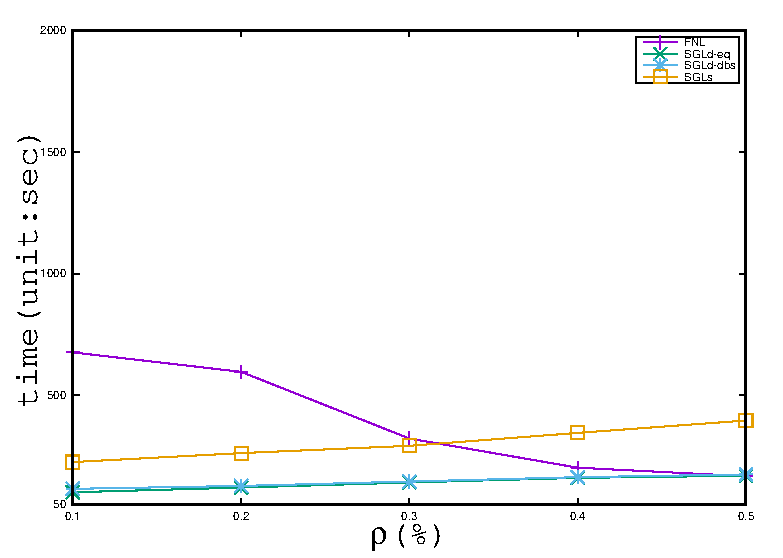
\includegraphics[width=2.2in]{time-v4k-e85k-a.eps}
         \label{fig:time-v4k-e85k:a}
    }
    \subfigure[DFS]{
        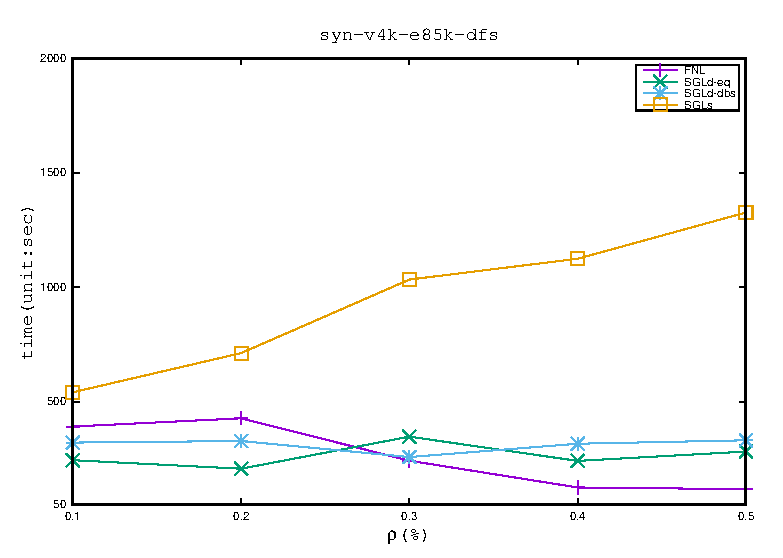
\includegraphics[width=2.2in]{time-v4k-e85k-b.eps}
        \label{fig:time-v4k-e85k:b}
    }
    \subfigure[BFS]{
       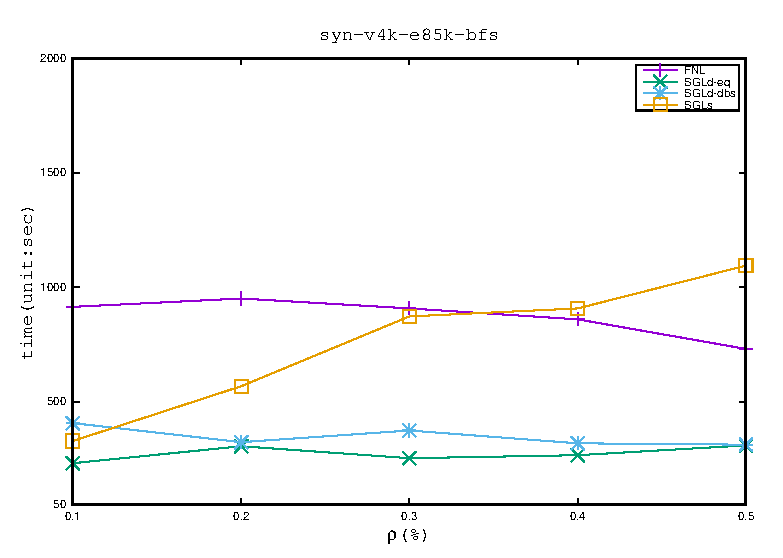
\includegraphics[width=2.2in]{time-v4k-e85k-c.eps}
       \label{fig:time-v4k-e85k:c}
    }
    \caption{Runtime VS. $\rho$ on syn-v4k-e85k Dataset, $k=4$}\label{fig:time-v4k-e85k}
\end{figure*}
\begin{figure*}[h]
    \centering
    \subfigure[RANDOM]{
        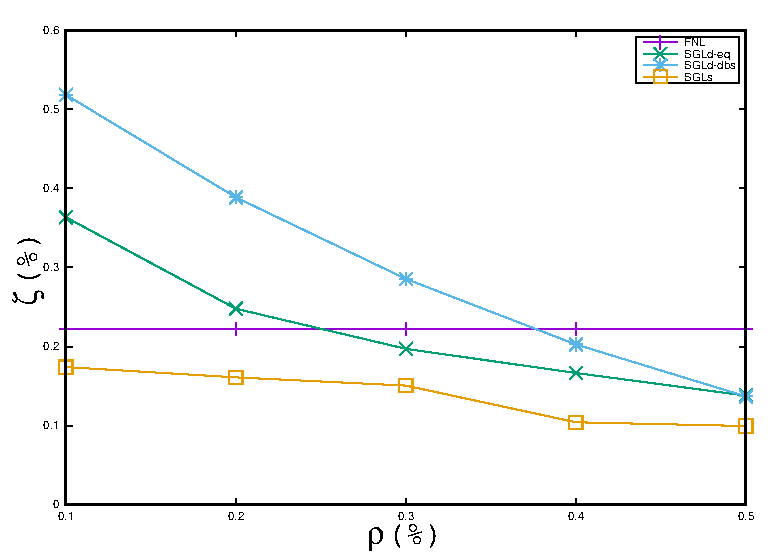
\includegraphics[width=2.2in]{cut-v4k-e85k-a.eps}
         \label{fig:cut-v4k-e85k:a}
    }
    \subfigure[DFS]{
        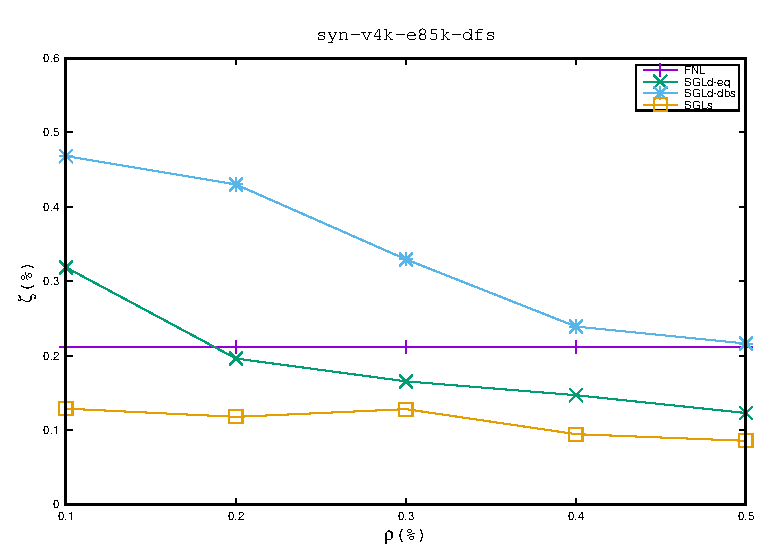
\includegraphics[width=2.2in]{cut-v4k-e85k-b.eps}
        \label{fig:cut-v4k-e85k:b}
    }
    \subfigure[BFS]{
       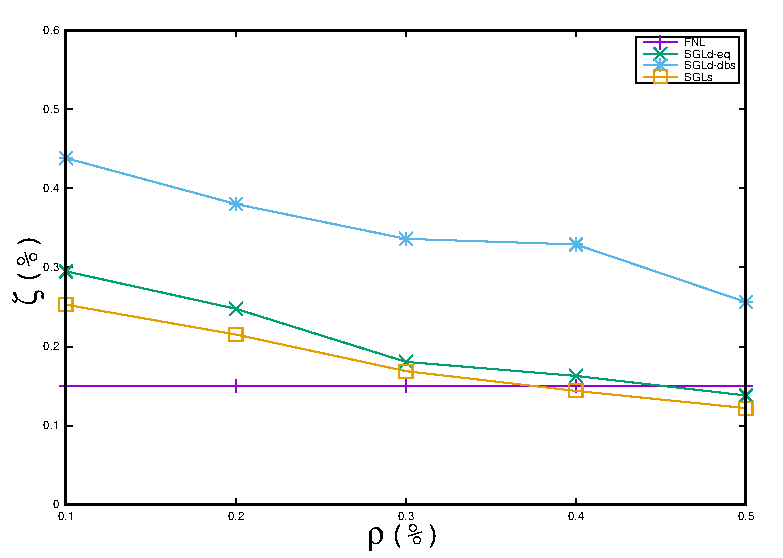
\includegraphics[width=2.2in]{cut-v4k-e85k-c.eps}
       \label{fig:cut-v4k-e85k:c}
    }
    \caption{ $\varsigma$ VS. $\rho$ on syn-v4k-e85k Dataset, $k=4$}\label{fig:cut-v4k-e85k}
\end{figure*}
\begin{figure*}[h]
    \centering
    \subfigure[RANDOM]{
        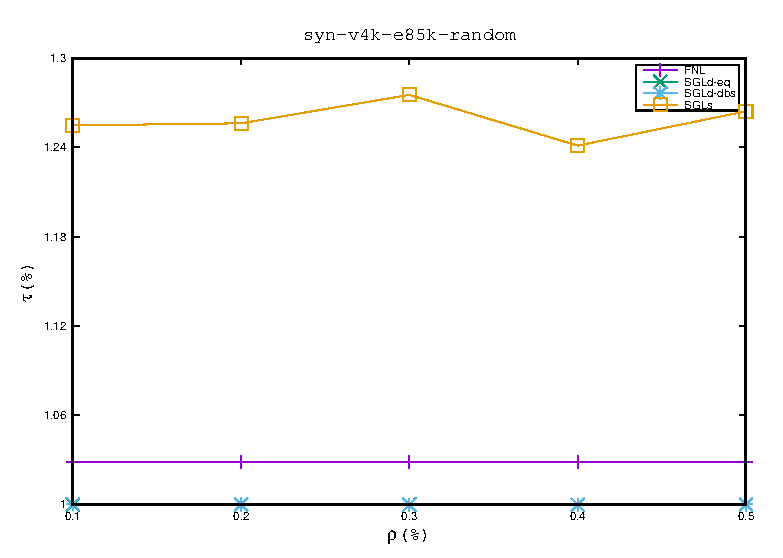
\includegraphics[width=2.2in]{maxload-v4k-e85k-a.eps}
         \label{fig:maxload-v4k-e85k:a}
    }
    \subfigure[DFS]{
        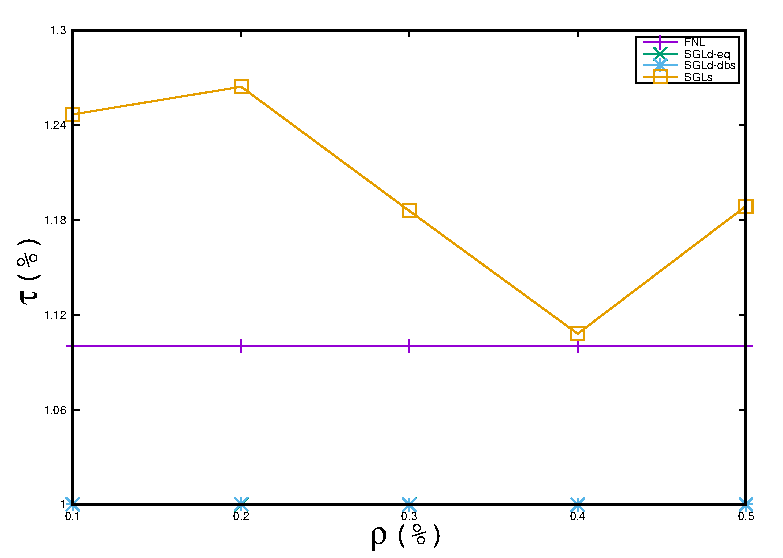
\includegraphics[width=2.2in]{maxload-v4k-e85k-b.eps}
        \label{fig:maxload-v4k-e85k:b}
    }
    \subfigure[BFS]{
       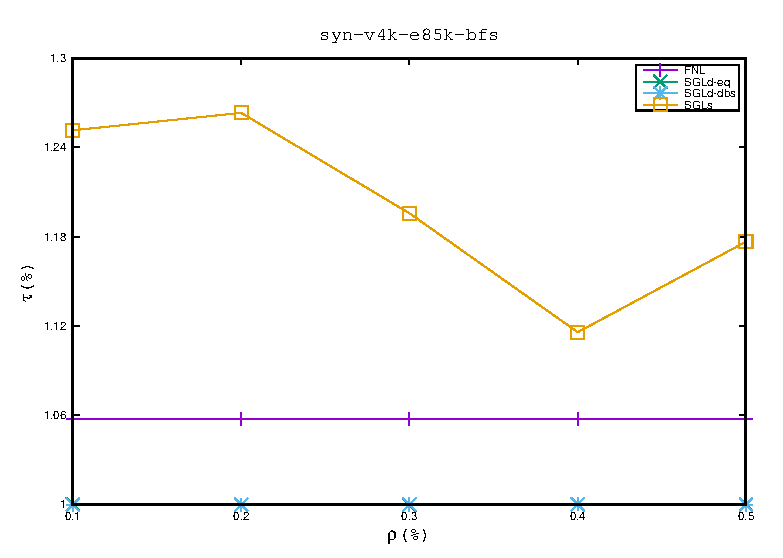
\includegraphics[width=2.2in]{maxload-v4k-e85k-c.eps}
       \label{fig:maxload-v4k-e85k:c}
    }
    \caption{ $\tau$ VS. $\rho$ on syn-v4k-e85k Dataset, $k=4$}\label{fig:maxload-v4k-e85k}
\end{figure*}
\begin{figure*}[h]
    \centering
    \subfigure[RANDOM]{
        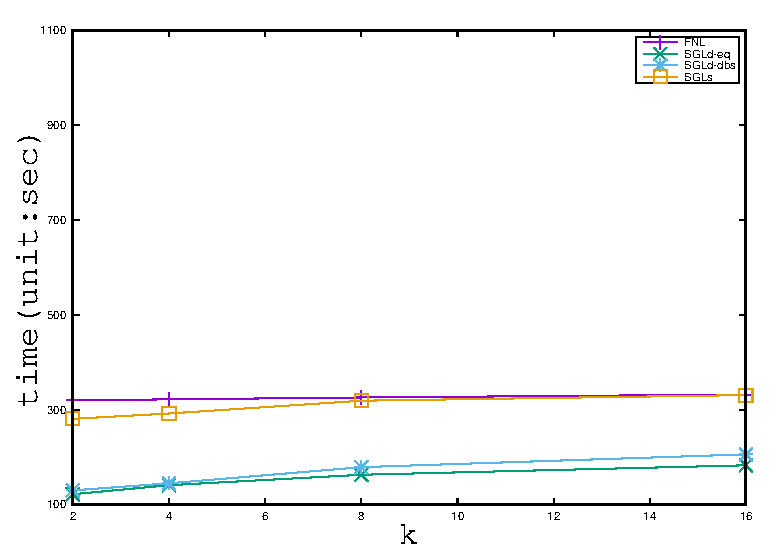
\includegraphics[width=2.2in]{time-to-k-v4k-e85k-a.eps}
         \label{fig:time-to-k-v4k-e85k:a}
    }
    \subfigure[DFS]{
        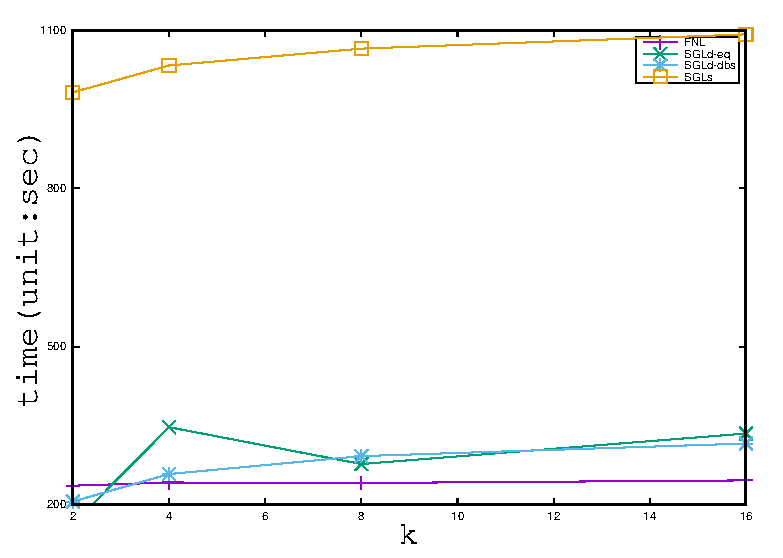
\includegraphics[width=2.2in]{time-to-k-v4k-e85k-b.eps}
        \label{fig:time-to-k-v4k-e85k:b}
    }
    \subfigure[BFS]{
       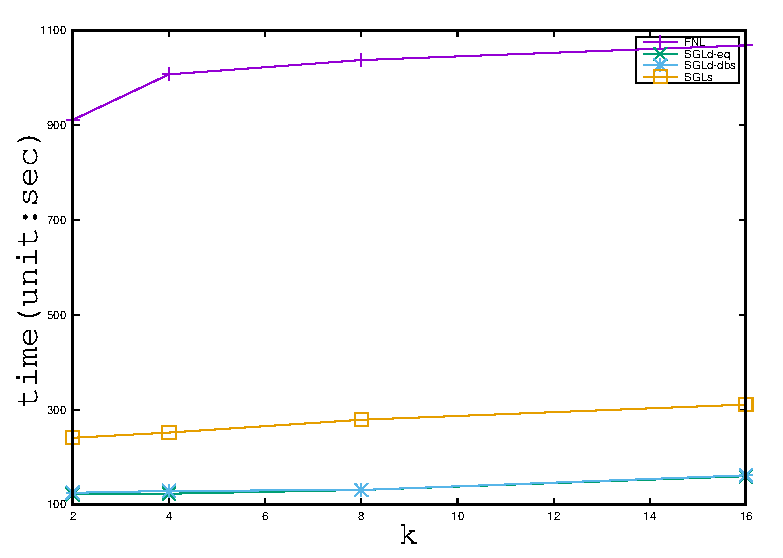
\includegraphics[width=2.2in]{time-to-k-v4k-e85k-c.eps}
       \label{fig:time-to-k-v4k-e85k:c}
    }
    \caption{ Time VS. $k$ on syn-v4k-e85k Dataset, $\rho=0.3$}\label{fig:time-to-k-v4k-e85k}
\end{figure*}
\begin{figure*}[h]
    \centering
    \subfigure[RANDOM]{
        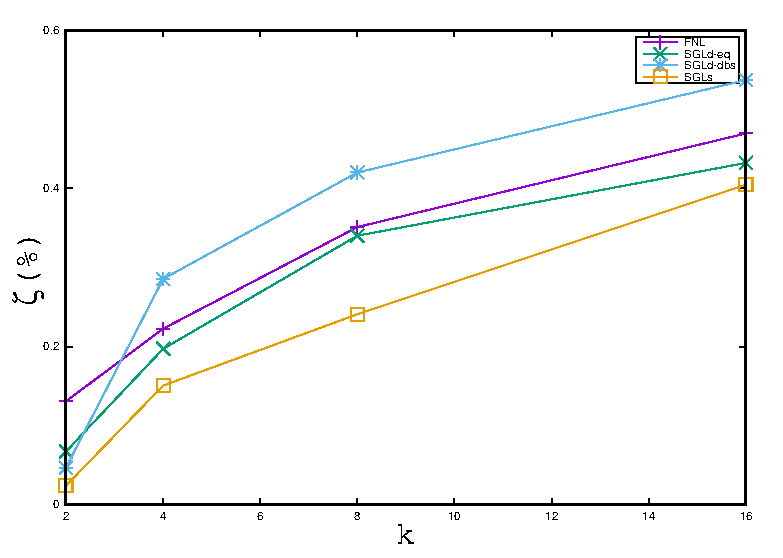
\includegraphics[width=2.2in]{cut-to-k-v4k-e85k-a.eps}
         \label{fig:cut-to-k-v4k-e85k:a}
    }
    \subfigure[DFS]{
        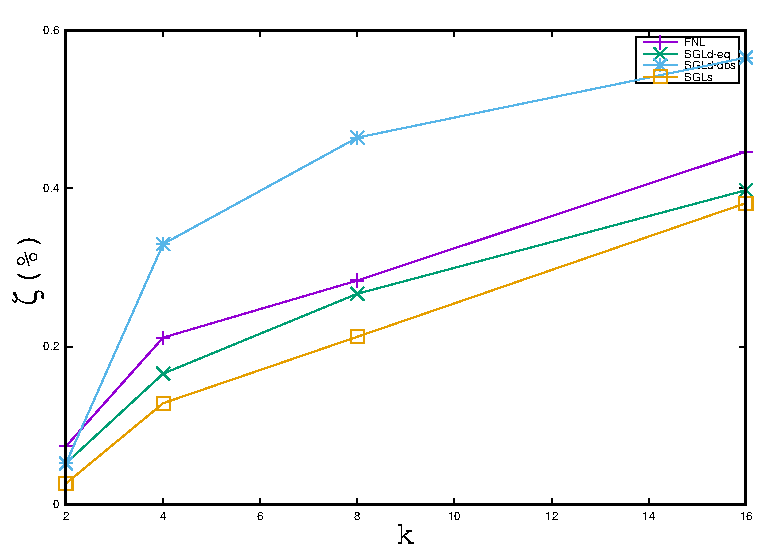
\includegraphics[width=2.2in]{cut-to-k-v4k-e85k-b.eps}
        \label{fig:cut-to-k-v4k-e85k:b}
    }
    \subfigure[BFS]{
       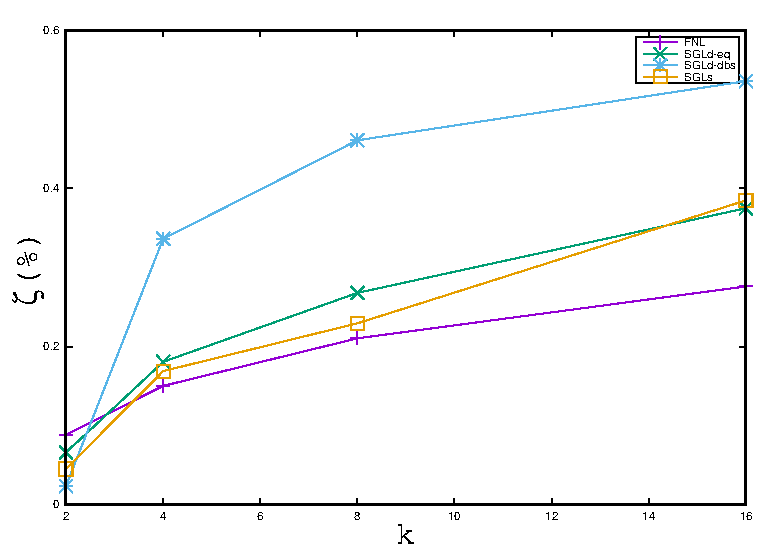
\includegraphics[width=2.2in]{cut-to-k-v4k-e85k-c.eps}
       \label{fig:cut-to-k-v4k-e85k:c}
    }
    \caption{ $\varsigma$ VS. $k$ on syn-v4k-e85k Dataset, $\rho=0.3$}\label{fig:cut-to-k-v4k-e85k}
\end{figure*}
\begin{figure*}[h]
    \centering
    \subfigure[RANDOM]{
        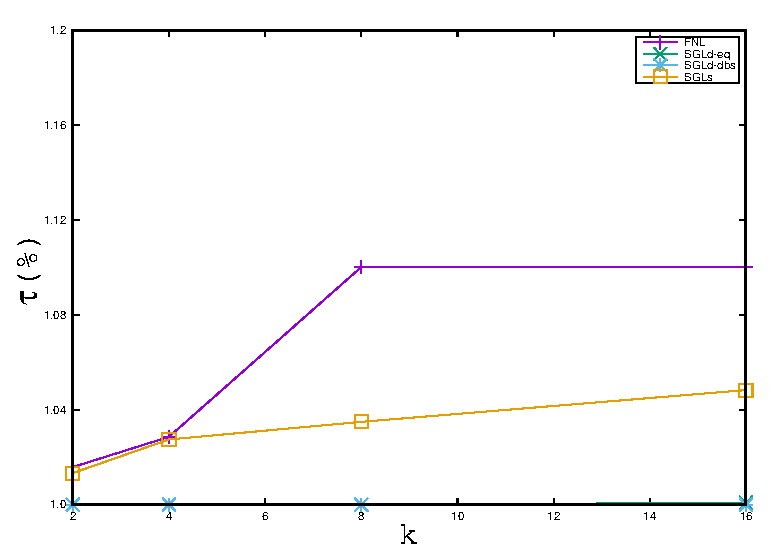
\includegraphics[width=2.2in]{maxload-to-k-v4k-e85k-a.eps}
         \label{fig:maxload-to-k-v4k-e85k:a}
    }
    \subfigure[DFS]{
        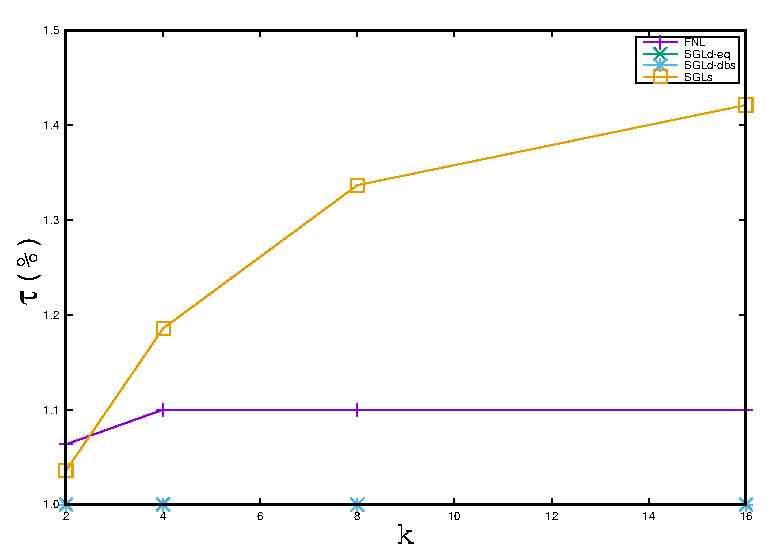
\includegraphics[width=2.2in]{maxload-to-k-v4k-e85k-b.eps}
        \label{fig:maxload-to-k-v4k-e85k:b}
    }
    \subfigure[BFS]{
       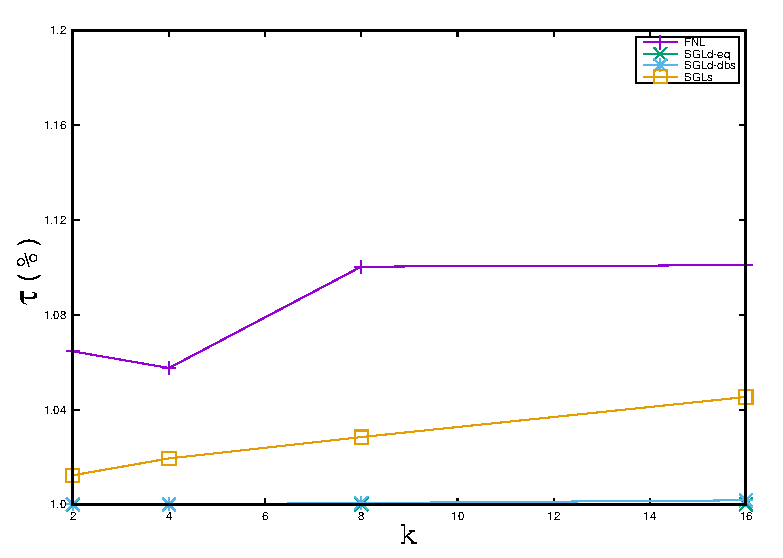
\includegraphics[width=2.2in]{maxload-to-k-v4k-e85k-c.eps}
       \label{fig:maxload-to-k-v4k-e85k:c}
    }
    \caption{ $\tau$ VS. $k$ on syn-v4k-e85k Dataset, $\rho=0.3$}\label{fig:maxload-to-k-v4k-e85k}
\end{figure*}
\begin{figure*}[h]
    \centering
    \subfigure[RANDOM]{
        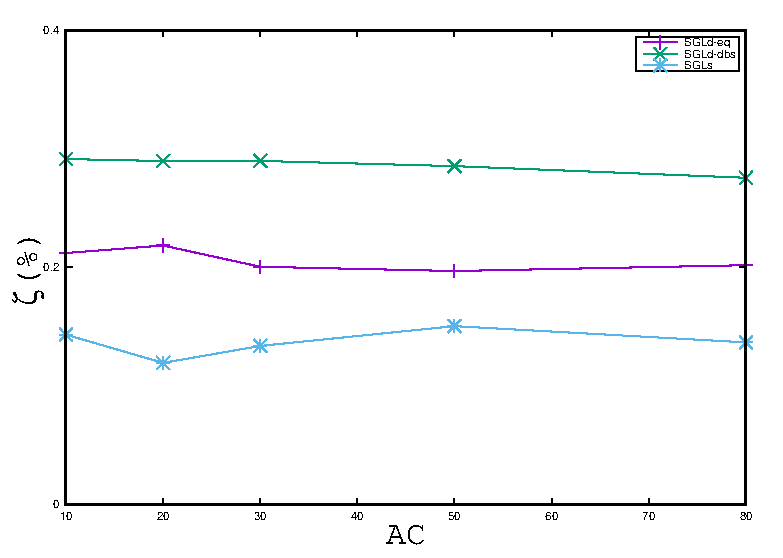
\includegraphics[width=2.2in]{cut-to-ac-v4k-e85k-a.eps}
         \label{fig:cut-to-ac-v4k-e85k:a}
    }
    \subfigure[DFS]{
        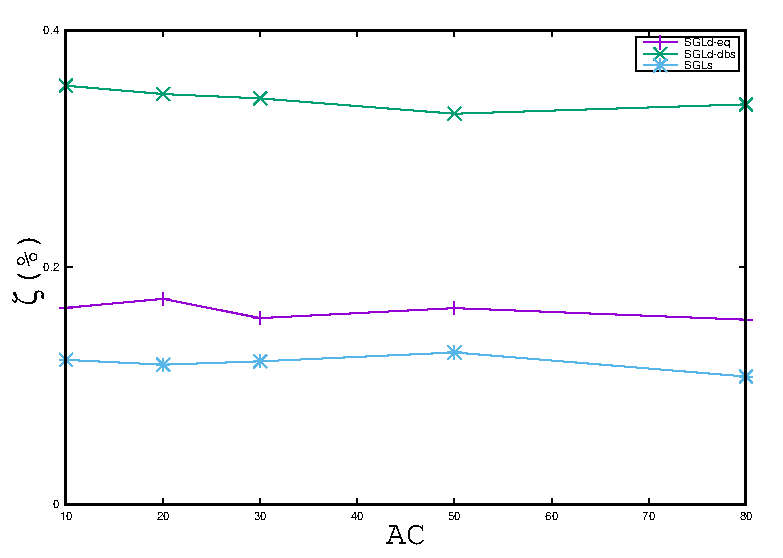
\includegraphics[width=2.2in]{cut-to-ac-v4k-e85k-b.eps}
        \label{fig:cut-to-ac-v4k-e85k:b}
    }
    \subfigure[BFS]{
       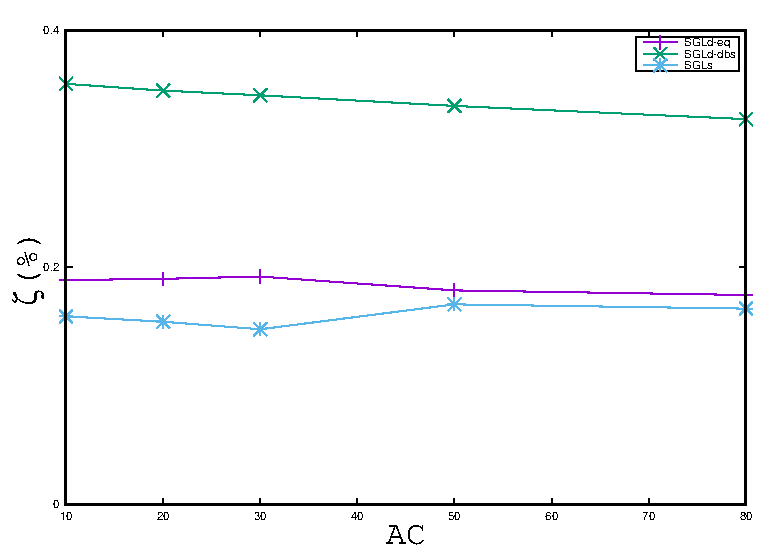
\includegraphics[width=2.2in]{cut-to-ac-v4k-e85k-c.eps}
       \label{fig:cut-to-ac-v4k-e85k:c}
    }
    \caption{ $\varsigma$ VS. $AC$ on syn-v4k-e85k Dataset, $\rho=0.3$, $k=4$}\label{fig:cut-to-ac-v4k-e85k}
\end{figure*}

\begin{figure*}[h]
    \centering
    \subfigure[RANDOM]{
        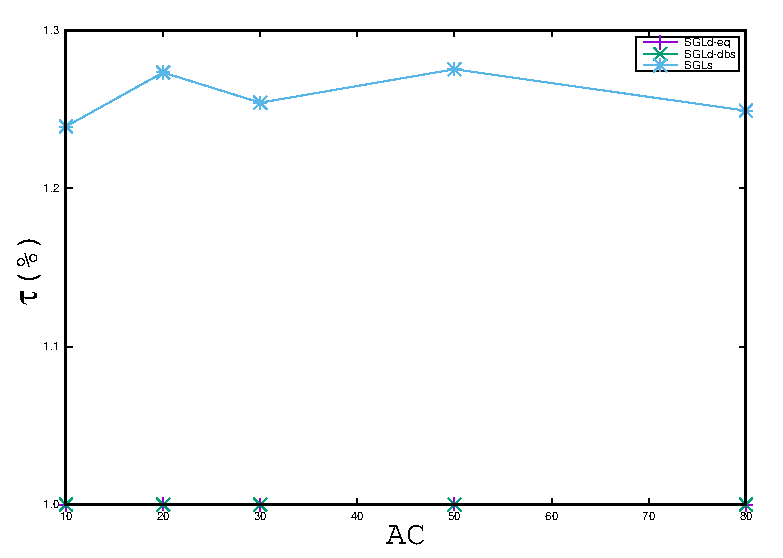
\includegraphics[width=2.2in]{maxload-to-ac-v4k-e85k-a.eps}
         \label{fig:maxload-to-ac-v4k-e85k:a}
    }
    \subfigure[DFS]{
        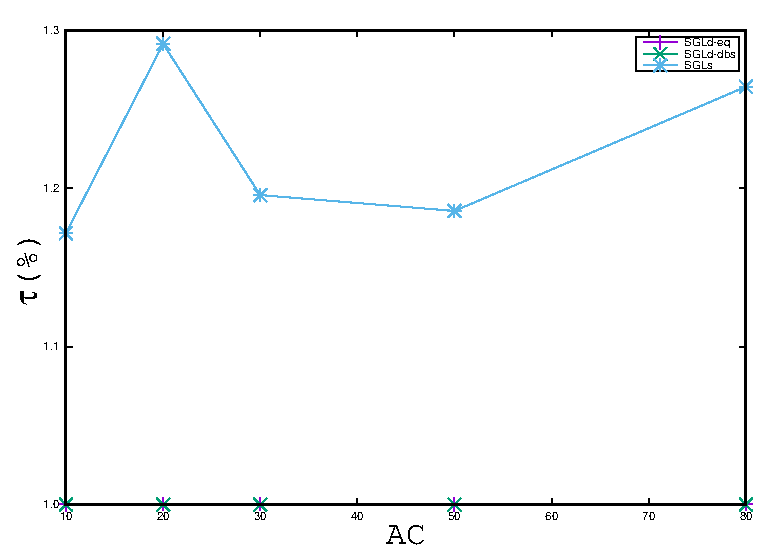
\includegraphics[width=2.2in]{maxload-to-ac-v4k-e85k-b.eps}
        \label{fig:maxload-to-ac-v4k-e85k:b}
    }
    \subfigure[BFS]{
       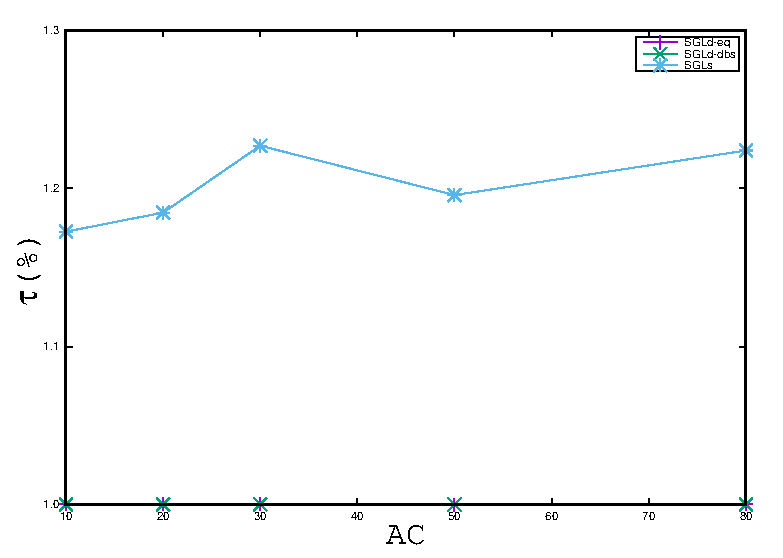
\includegraphics[width=2.2in]{maxload-to-ac-v4k-e85k-c.eps}
       \label{fig:maxload-to-ac-v4k-e85k:c}
    }
    \caption{ $\tau$ VS. $AC$ on syn-v4k-e85k Dataset, $\rho=0.3$, $k=4$}\label{fig:maxload-to-ac-v4k-e85k}
\end{figure*}

\clearpage % fix bug: too many unprocessed float

\begin{comment}
\begin{figure*}[htbp]
    \centering
    \subfigure[RANDOM]{
        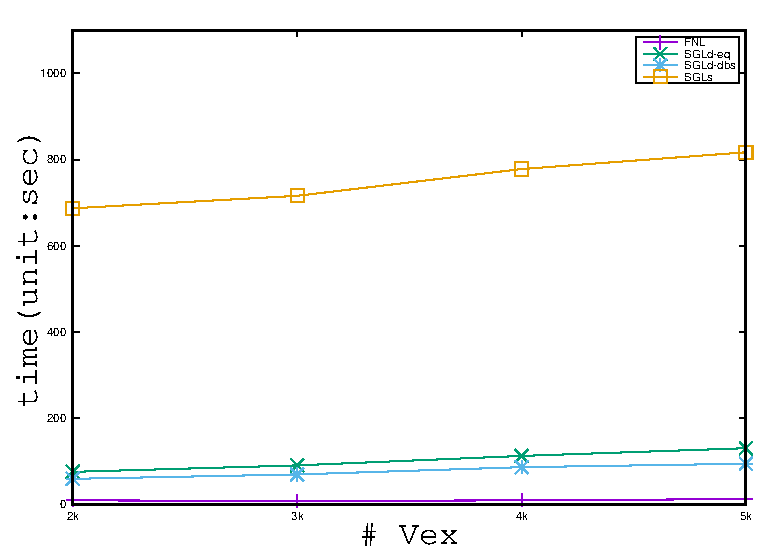
\includegraphics[width=2.2in]{time-v-change-e80k-a.eps}
         \label{fig:time-v-change-e80k:a}
    }
    \subfigure[DFS]{
        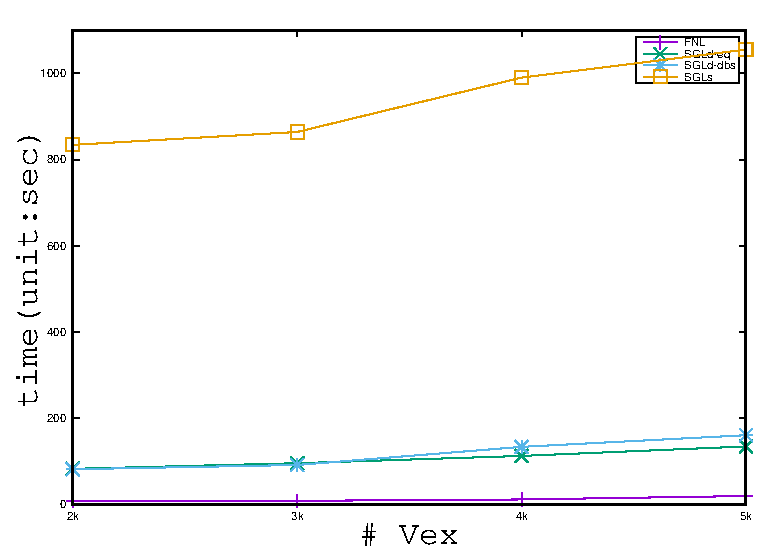
\includegraphics[width=2.2in]{time-v-change-e80k-b.eps}
        \label{fig:time-v-change-e80k:b}
    }
    \subfigure[BFS]{
       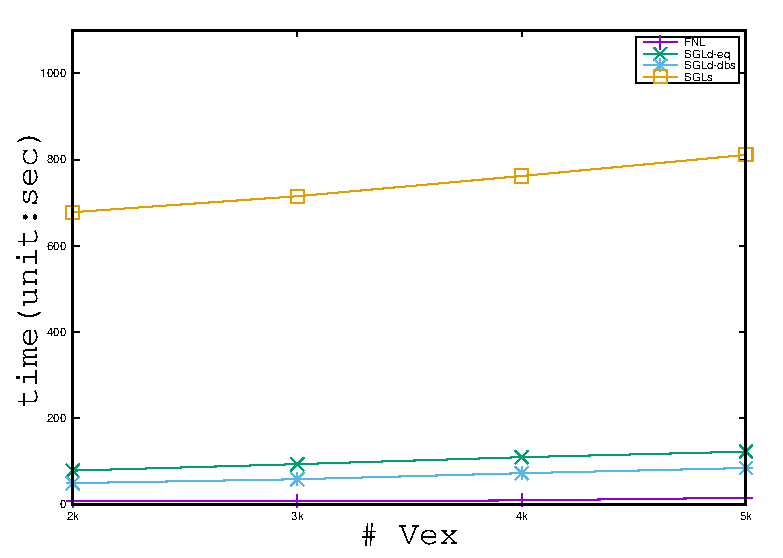
\includegraphics[width=2.2in]{time-v-change-e80k-c.eps}
       \label{fig:time-v-change-e80k:c}
    }
    \caption{ Time VS. $\# Vex$, $\rho=0.3$, $k=4$, $AC=50$}\label{fig:time-v-change-e80k}
\end{figure*}
\begin{figure*}[htbp]
    \centering
    \subfigure[RANDOM]{
        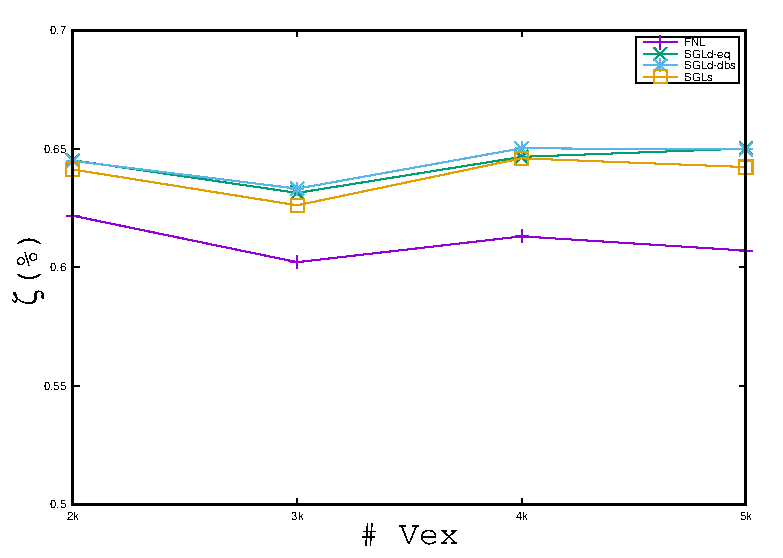
\includegraphics[width=2.2in]{cut-v-change-e80k-a.eps}
         \label{fig:cut-v-change-e80k:a}
    }
    \subfigure[DFS]{
        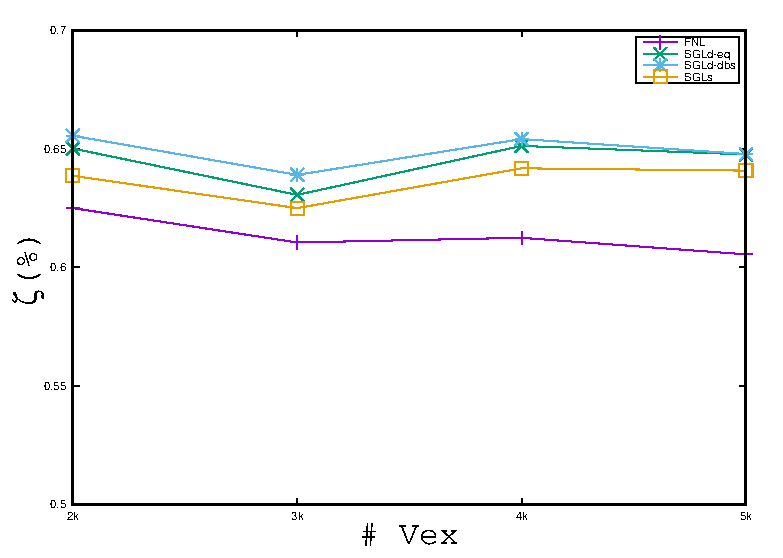
\includegraphics[width=2.2in]{cut-v-change-e80k-b.eps}
        \label{fig:cut-v-change-e80k:b}
    }
    \subfigure[BFS]{
       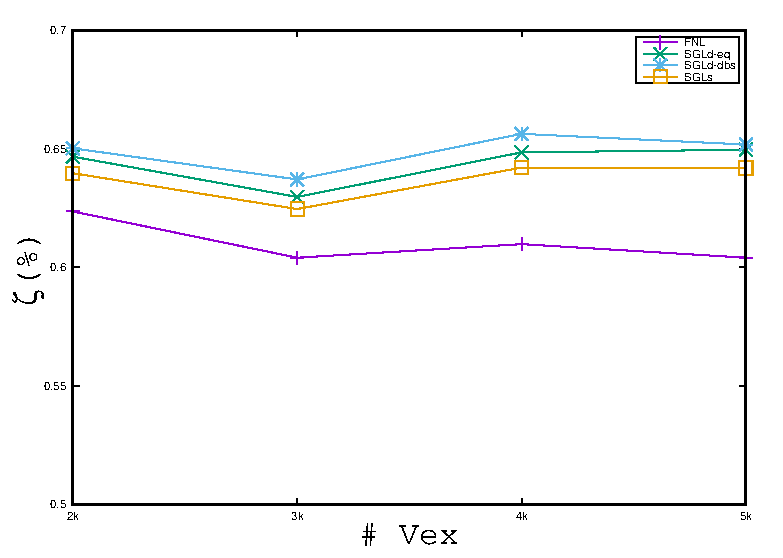
\includegraphics[width=2.2in]{cut-v-change-e80k-c.eps}
       \label{fig:cut-v-change-e80k:c}
    }
    \caption{ $\varsigma$ VS. $\# Vex$, $\rho=0.3$, $k=4$, $AC=50$}\label{fig:cut-v-change-e80k}
\end{figure*}
\begin{figure*}[htbp]
    \centering
    \subfigure[RANDOM]{
        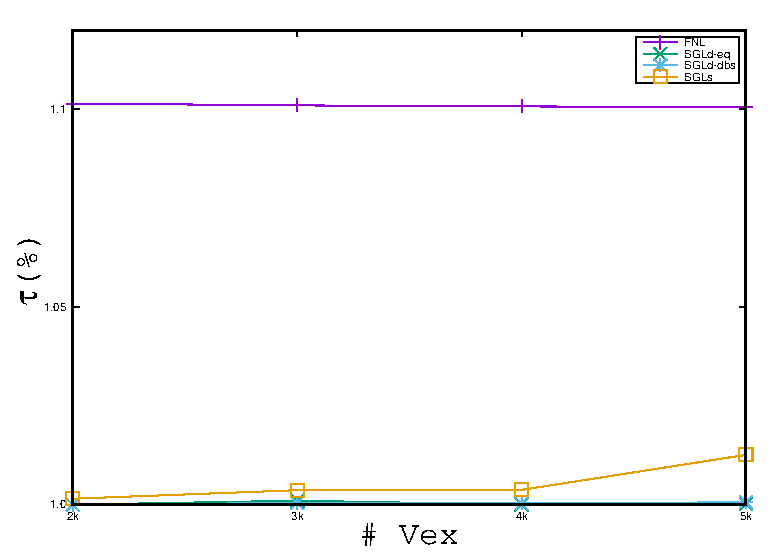
\includegraphics[width=2.2in]{maxload-v-change-e80k-a.eps}
         \label{fig:maxload-v-change-e80k:a}
    }
    \subfigure[DFS]{
        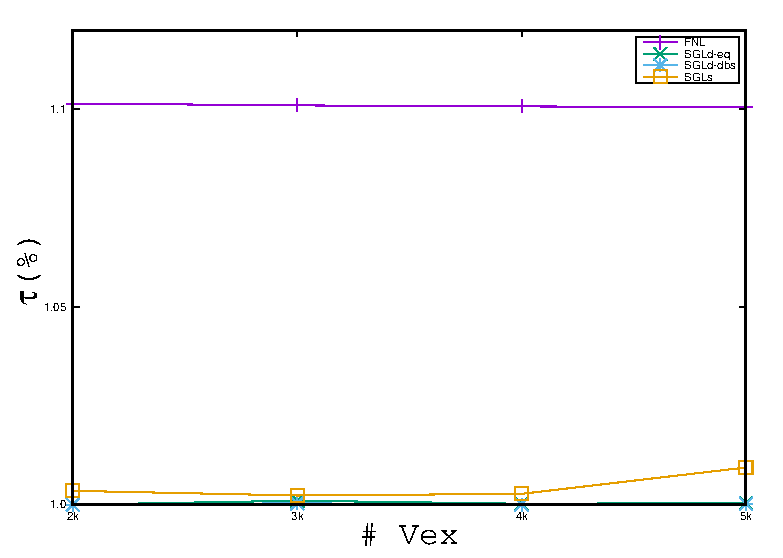
\includegraphics[width=2.2in]{maxload-v-change-e80k-b.eps}
        \label{fig:maxload-v-change-e80k:b}
    }
    \subfigure[BFS]{
       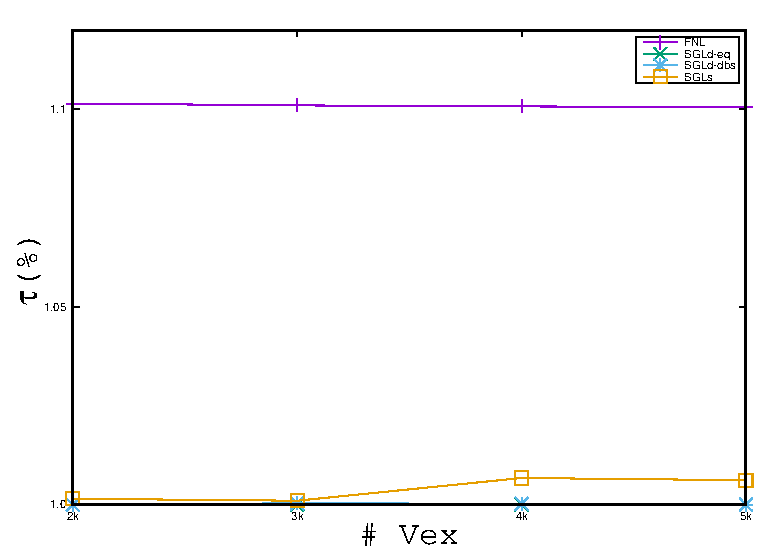
\includegraphics[width=2.2in]{maxload-v-change-e80k-c.eps}
       \label{fig:maxload-v-change-e80k:c}
    }
    \caption{ $\tau$ VS. $\# Vex$, $\rho=0.3$, $k=4$, $AC=50$}\label{fig:maxload-v-change-e80k}
\end{figure*}

\begin{figure*}[htbp]
    \centering
    \subfigure[RANDOM]{
        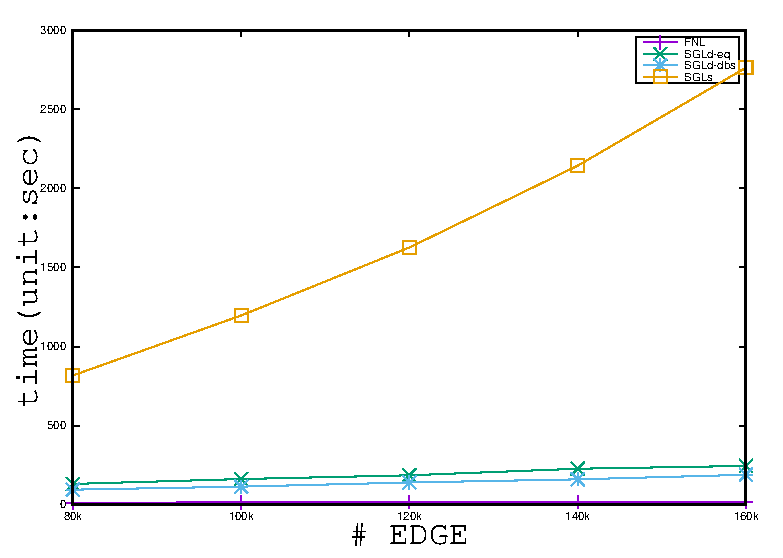
\includegraphics[width=2.2in]{time-v5k-e-change-a.eps}
         \label{fig:time-v5k-e-change:a}
    }
    \subfigure[DFS]{
        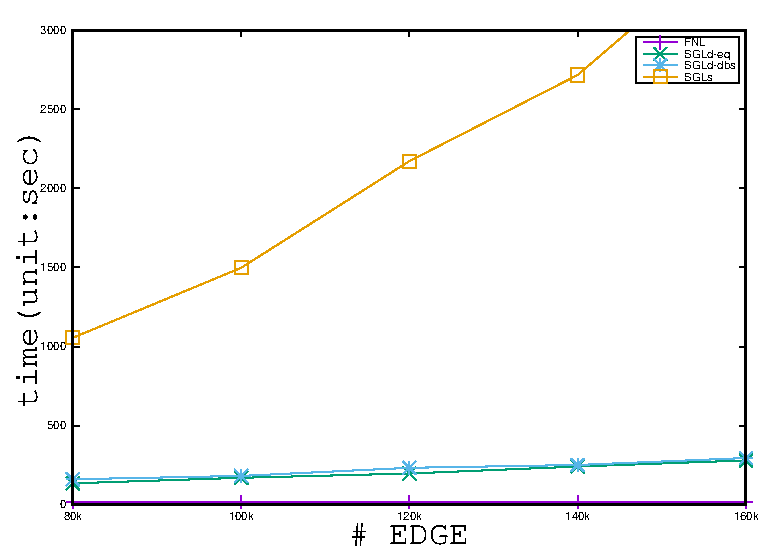
\includegraphics[width=2.2in]{time-v5k-e-change-b.eps}
        \label{fig:time-v5k-e-change:b}
    }
    \subfigure[BFS]{
       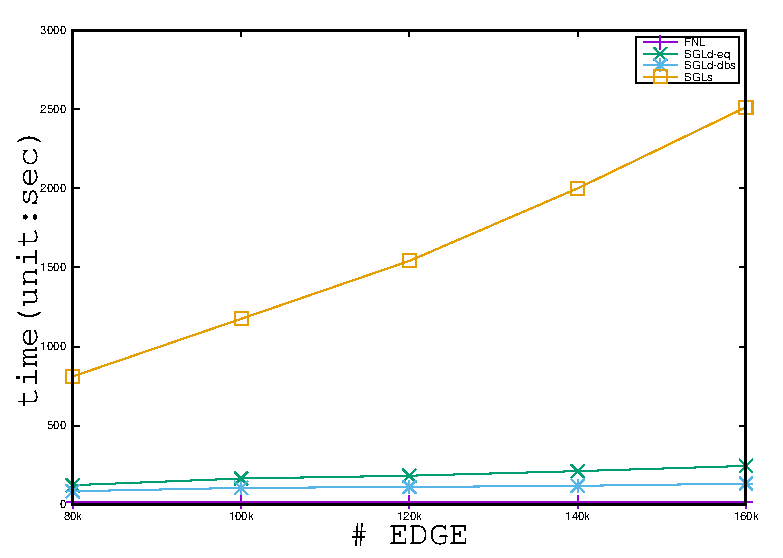
\includegraphics[width=2.2in]{time-v5k-e-change-c.eps}
       \label{fig:time-v5k-e-change:c}
    }
    \caption{ Time VS. $\#\ EDGE$, $\rho=0.3$, $k=4$, $AC=50$}\label{fig:time-v5k-e-change}
\end{figure*}
\begin{figure*}[htbp]
    \centering
    \subfigure[RANDOM]{
        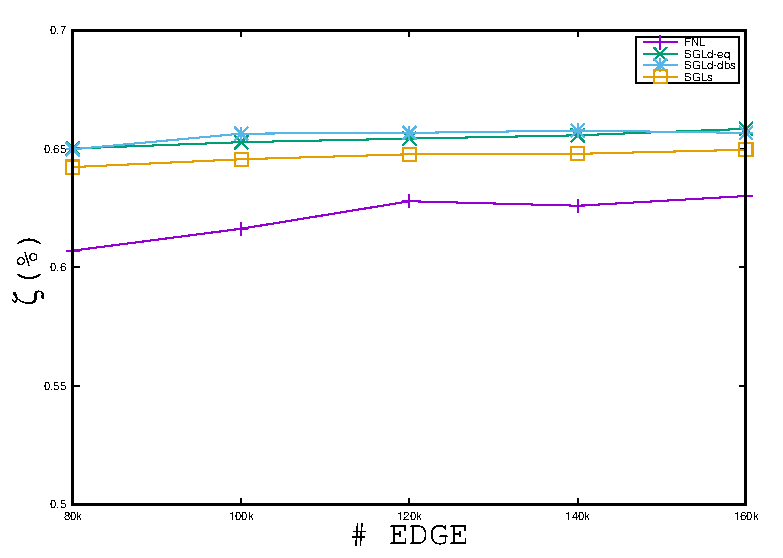
\includegraphics[width=2.2in]{cut-v5k-e-change-a.eps}
         \label{fig:cut-v5k-e-change:a}
    }
    \subfigure[DFS]{
        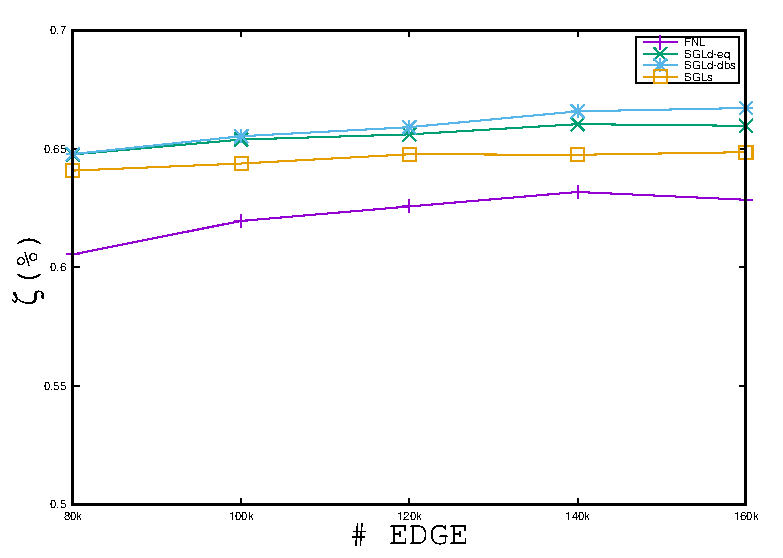
\includegraphics[width=2.2in]{cut-v5k-e-change-b.eps}
        \label{fig:cut-v5k-e-change:b}
    }
    \subfigure[BFS]{
       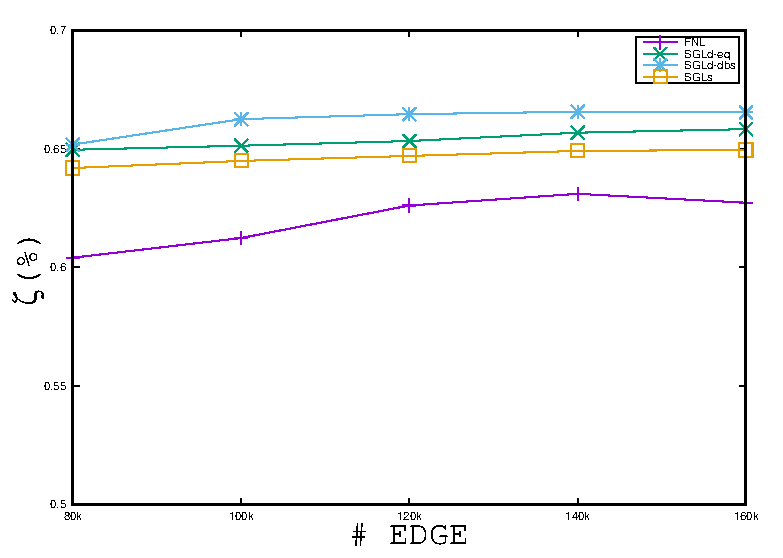
\includegraphics[width=2.2in]{cut-v5k-e-change-c.eps}
       \label{fig:cut-v5k-e-change:c}
    }
    \caption{ $\varsigma$ VS. $\#\ EDGE$, $\rho=0.3$, $k=4$, $AC=50$}\label{fig:cut-v5k-e-change}
\end{figure*}
\begin{figure*}[htbp]
    \centering
    \subfigure[RANDOM]{
        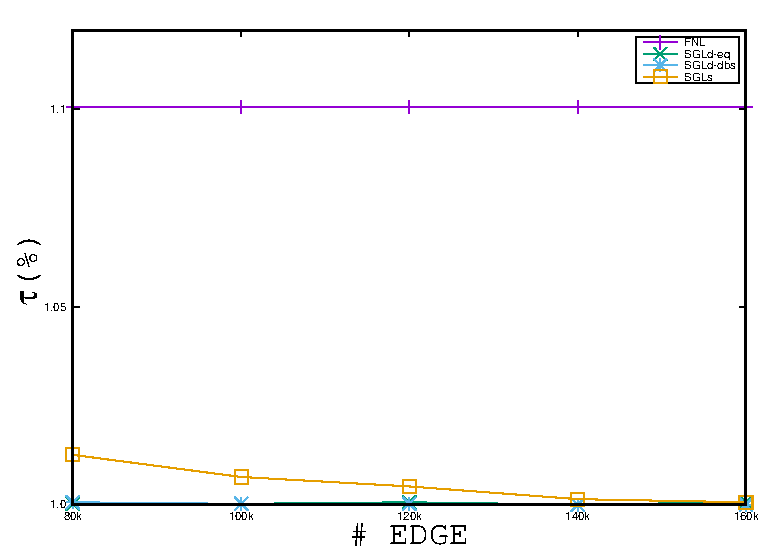
\includegraphics[width=2.2in]{maxload-v5k-e-change-a.eps}
         \label{fig:maxload-v5k-e-change:a}
    }
    \subfigure[DFS]{
        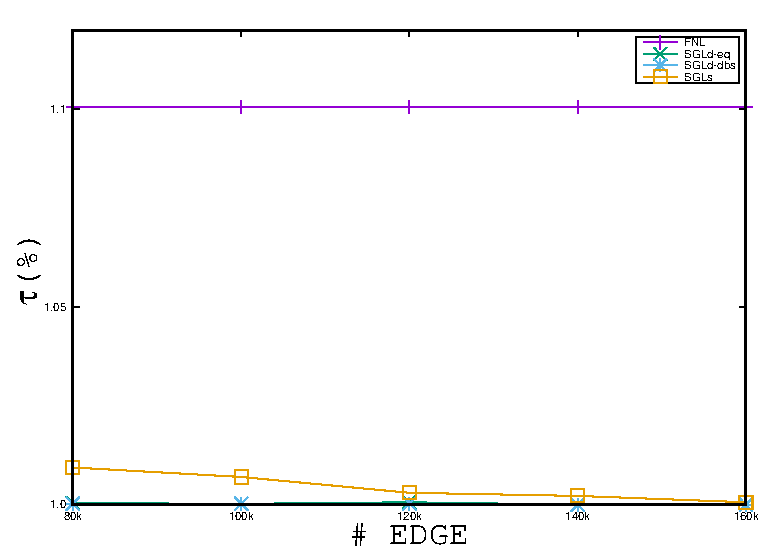
\includegraphics[width=2.2in]{maxload-v5k-e-change-b.eps}
        \label{fig:maxload-v5k-e-change:b}
    }
    \subfigure[BFS]{
       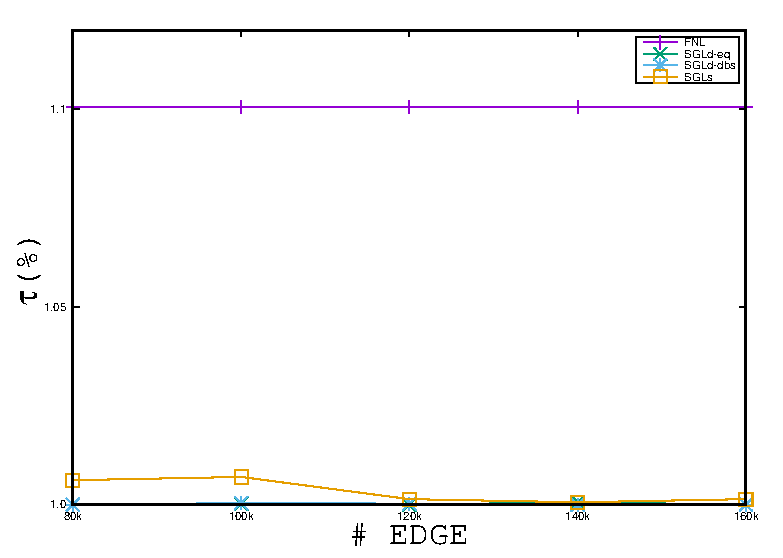
\includegraphics[width=2.2in]{maxload-v5k-e-change-c.eps}
       \label{fig:maxload-v5k-e-change:c}
    }
    \caption{ $\tau$ VS. $\#\ EDGE$, $\rho=0.3$, $k=4$, $AC=50$}\label{fig:maxload-v5k-e-change}
\end{figure*}
\clearpage
\end{comment}
\section{Conclusions}
In this work we provide a new perspective on the well studied problem of balanced graph partitioning. We introduce the concept of expectation of error gain to measure the quality of partitions instead of edges cut. The theoretical analysis on the bound of gain expectation is given as the base of building the representative graph by streaming sampling edges.  We design two efficient algorithms to load the big graph into distributed system in manner of graph partitions: \textbf{SGLd}, two-pass disk-based graph partitioning and \textbf{SGLs}, one-pass streaming graph partitioning. We also demonstrated these two methods can dramatically improve the efficiency of partitioning with small memory limitation and show the comparable performance of edge-cut and balance in comparison to the state-in-the-art algorithms
%\section{Acknowledgments}
\bibliographystyle{abbrv}
\bibliography{sigproc}
\balancecolumns
\end{document}
